\documentclass[11pt]{article}

%%%%%%%%%%%%%%%%%%%%%%%%%%%%%%%%%%%%%%%%%%%%%%%%%%%%%%%%%%%%%%%%%%%%
%%%%%%%%%%%%%%%%%%%%%%%%%%%%%%%%%%%%%%%%%%%%%%%%%%%%%%%%%%%%%%%%%%%%
% various packages
\usepackage[a4paper,top=2.25cm,bottom=2.25cm,left=2.75cm,right=2.75cm,marginparwidth=2cm,hmarginratio=1:1]{geometry}
\usepackage[USenglish]{babel}
\usepackage{indentfirst} % We should be able to know if this is a new paragraph, without context info (section etc).
\usepackage{relsize}
\usepackage{engord} % 1 -> 1st, 2 -> 2nd, etc
\usepackage{kantlipsum}
\usepackage{graphicx}
%% Using wrapfigure of course requires finetuning, so it is not robust to layout or content changes.
%% The result is aesthetically pleasing, though.
%\usepackage{wrapfig}
\usepackage{mparhack}
\usepackage[
  stable,
%  symbol*,
]{footmisc}
\usepackage{tikz-cd}
\usepackage{rotating}
\usepackage{pdflscape}
\usepackage{amsmath}
\usepackage{bclogo}
\usepackage[
  %font=it,
  labelfont=bf
]{caption}
\usepackage{float}
\usepackage{xspace}
\usepackage{termsim}
% For some reason, you must use fontawesome _after_ termsim
\usepackage{fontawesome} % https://ctan.org/pkg/fontawesome
\usepackage{datetime2}

%%%%%%%%%%%%%%%%%%%%%%%%%%%%%%%%%%%%%%%%%%%%%%%%%%%%%%%%%%%%%%%%%%%%
%%%%%%%%%%%%%%%%%%%%%%%%%%%%%%%%%%%%%%%%%%%%%%%%%%%%%%%%%%%%%%%%%%%%
% type inference rules
\usepackage[inference]{semantic}

% inference rule
\newcommand{\infrule}[3]{\begin{tabular}{ll} \fbox{\textsf{#1}} & \inference{#2}{#3} \end{tabular}}
%%%%%%%%%%%%%%%%%%%%%%%%%%%%%%%%%%%%%%%%%%%%%%%%%%%%%%%%%%%%%%%%%%%%
%%%%%%%%%%%%%%%%%%%%%%%%%%%%%%%%%%%%%%%%%%%%%%%%%%%%%%%%%%%%%%%%%%%%
% table of contents
\usepackage[toc]{multitoc}
\setlength{\columnseprule}{1pt}

\usepackage{tocloft}
\renewcommand{\cftsecleader}{\cftdotfill{\cftdotsep}}

\setcounter{tocdepth}{2}
%%%%%%%%%%%%%%%%%%%%%%%%%%%%%%%%%%%%%%%%%%%%%%%%%%%%%%%%%%%%%%%%%%%%
%%%%%%%%%%%%%%%%%%%%%%%%%%%%%%%%%%%%%%%%%%%%%%%%%%%%%%%%%%%%%%%%%%%%
% links and references
\newcommand{\TheTitleA}{Denotational semantics for the masses}
\newcommand{\TheTitleB}{Calculating a Ledger, among other things}
\newcommand{\TheTitle}{\TheTitleA: \TheTitleB}
\newcommand{\TheOneSpec}{One spec to rule them all, one spec to find them, one spec to bring them all and in the darkness bind them}

\usepackage[%
  final,%
  backref=page,pagebackref=true,%
  colorlinks=true,%
  allcolors=blue,%
  bookmarksopen=true,%
  bookmarksnumbered=true,%
  pdfauthor={Christos KK Loverdos},%
  pdftitle={\TheTitle},%
  pdfsubject={\TheTitle. \TheOneSpec},%
  pdfkeywords={semantics, denotational semantics, tagless-final, compilers, AST, ADT, GADT, abstract syntax tree, DSL, domain-specific language, Scala, OCaml, Haskell, type inference},% 
]{hyperref}
\usepackage[nospace]{varioref}

\renewcommand{\vref}[1]{\autoref{#1} \vpageref{#1}}{}
%%%%%%%%%%%%%%%%%%%%%%%%%%%%%%%%%%%%%%%%%%%%%%%%%%%%%%%%%%%%%%%%%%%%
%%%%%%%%%%%%%%%%%%%%%%%%%%%%%%%%%%%%%%%%%%%%%%%%%%%%%%%%%%%%%%%%%%%%
%% fonts
%% See also https://r2src.github.io/top10fonts/
%%
\usepackage{amsfonts}
\usepackage{amsmath}
\usepackage{amstext}

% pdflatex
%\usepackage{fontenc}
%\usepackage{tgpagella}
%\usepackage[utopia]{mathdesign} % more modern than \usepackage{utopia}

% xelatex
\usepackage{fontspec}
\usepackage[math-style=ISO,bold-style=ISO]{unicode-math}
\defaultfontfeatures{Ligatures=TeX} %Numbers=OldStyle

\setmainfont{Libertinus Serif}
\setsansfont{Libertinus Sans}
\setmathfont{Libertinus Math}
\setmonofont{Libertinus Mono}
%%%%%%%%%%%%%%%%%%%%%%%%%%%%%%%%%%%%%%%%%%%%%%%%%%%%%%%%%%%%%%%%%%%%
%%%%%%%%%%%%%%%%%%%%%%%%%%%%%%%%%%%%%%%%%%%%%%%%%%%%%%%%%%%%%%%%%%%%
%% colors
\usepackage{xcolor}
\definecolor{kkRed1}{RGB}{255,219,219}
\definecolor{kkRed2}{RGB}{230,197,197}
\definecolor{kkRed3}{RGB}{204,175,175}
\definecolor{kkRed4}{RGB}{178,153,153}
\definecolor{kkRed5}{RGB}{153,131,131}

\definecolor{kkGreen1}{RGB}{219,255,219}
\definecolor{kkGreen2}{RGB}{197,230,197}
\definecolor{kkGreen3}{RGB}{175,204,175}
\definecolor{kkGreen4}{RGB}{153,178,153}
\definecolor{kkGreen5}{RGB}{131,153,131}

\definecolor{kkBlue1}{RGB}{219,219,255}
\definecolor{kkBlue2}{RGB}{197,197,230}
\definecolor{kkBlue3}{RGB}{175,175,204}
\definecolor{kkBlue4}{RGB}{153,153,178}
\definecolor{kkBlue5}{RGB}{131,131,153}
%%%%%%%%%%%%%%%%%%%%%%%%%%%%%%%%%%%%%%%%%%%%%%%%%%%%%%%%%%%%%%%%%%%%
%%%%%%%%%%%%%%%%%%%%%%%%%%%%%%%%%%%%%%%%%%%%%%%%%%%%%%%%%%%%%%%%%%%%
%% frames, boxes, code blocks
\usepackage{mdframed}

% https://ctan.org/pkg/minted
\usepackage{minted}
\setminted{fontsize=\footnotesize,baselinestretch=0.7}
\setminted{linenos=false}
\setminted{style=default}

% https://ctan.org/pkg/tcolorbox
\usepackage{tcolorbox}
\tcbuselibrary{all}
%\tcbset{default minted options={linenos,autogobble,numbersep=2mm}}
\tcbset{beamer,enhanced}
\tcbset{colback=white,colframe=kkBlue5,boxrule=0.2pt,left=5mm}
% colback=yellow!10!white

\newcommand{\Scala}[1]{\mintinline{scala}|#1|}
\newcommand{\ScalaI}[1]{\mintinline{scala}|#1|}
\newcommand{\ScalaB}[1]{\mint{scala}|#1|}

\newcommand{\TextI}[1]{\mintinline{text}|#1|}

\newtcblisting{ScalaBlock}{
  listing only,
  listing engine=minted,
  minted language=scala,
  minted options={
    linenos,
    autogobble,
    numbersep=2mm,
  },
  overlay={\begin{tcbclipinterior}\fill[kkGreen1] (frame.south west) rectangle ([xshift=5mm]frame.north west);\end{tcbclipinterior}}
}

\newtcblisting{ScalaBlockLines}{
  listing only,
  listing engine=minted,
  minted language=scala,
  minted options={
    linenos,
    autogobble,
    numbersep=2mm,
  },
  frame hidden,
  no shadow
}

\newtcblisting{ScalaBlockSimple}{
  listing only,
  listing engine=minted,
  minted language=scala,
  minted options={
    autogobble,    
  },
  frame hidden,
  no shadow
}



\mdfdefinestyle{kkmdabstract}{%
    linecolor=kkRed5, linewidth=0.8pt,
    backgroundcolor=kkRed1,
    leftline=false, rightline=false,
    innertopmargin=0.20cm, innerbottommargin=0.20cm,
    innerleftmargin=0.20cm, innerrightmargin=0.20cm,
}
%%%%%%%%%%%%%%%%%%%%%%%%%%%%%%%%%%%%%%%%%%%%%%%%%%%%%%%%%%%%%%%%%%%%
%%%%%%%%%%%%%%%%%%%%%%%%%%%%%%%%%%%%%%%%%%%%%%%%%%%%%%%%%%%%%%%%%%%%
% fancy stuff on pages
\usepackage{coffee}
% In the presence of tcolobox, eso-pic seems to be more robust than draftwatermark
\usepackage{eso-pic}

\AddToShipoutPictureFG{%
\begin{tikzpicture}[overlay,remember picture]
\path (current page.south west) -- (current page.north east)
 node[midway,scale=12,color=gray,sloped,opacity=0.2] {\textbf{DRAFT}};
\end{tikzpicture}
}

%%%%%%%%%%%%%%%%%%%%%%%%%%%%%%%%%%%%%%%%%%%%%%%%%%%%%%%%%%%%%%%%%%%%
%%%%%%%%%%%%%%%%%%%%%%%%%%%%%%%%%%%%%%%%%%%%%%%%%%%%%%%%%%%%%%%%%%%%
% Todos (need the colors, hence comes later)
\usepackage[
  colorinlistoftodos,
  loadshadowlibrary,shadow,
  textwidth=1.17\marginparwidth,
  backgroundcolor=kkGreen1,
  bordercolor=kkGreen4,
  linecolor=kkGreen3,
  textsize=footnotesize,
]{todonotes}

\setuptodonotes{%
  %fancyline,
}

%%%%%%%%%%%%%%%%%%%%%%%%%%%%%%%%%%%%%%%%%%%%%%%%%%%%%%%%%%%%%%%%%%%%
%%%%%%%%%%%%%%%%%%%%%%%%%%%%%%%%%%%%%%%%%%%%%%%%%%%%%%%%%%%%%%%%%%%%
% margin notes
\newcommand{\OneTwoThreeX}[1]{\marginpar{\faCubes{ \smaller #1}}\xspace}
\newcommand{\OneTwoThree}{\OneTwoThreeX{}}
\newcommand{\FirstEtcX}[1]{\marginpar{\faCube{ \smaller #1}}\xspace}
\newcommand{\FirstEtc}{\FirstEtcX{}}

%%%%%%%%%%%%%%%%%%%%%%%%%%%%%%%%%%%%%%%%%%%%%%%%%%%%%%%%%%%%%%%%%%%%
%%%%%%%%%%%%%%%%%%%%%%%%%%%%%%%%%%%%%%%%%%%%%%%%%%%%%%%%%%%%%%%%%%%%
% underlying empty space
\newcommand{\uempty}[1][x]{\underline{\phantom{#1}}}

%%%%%%%%%%%%%%%%%%%%%%%%%%%%%%%%%%%%%%%%%%%%%%%%%%%%%%%%%%%%%%%%%%%%
%%%%%%%%%%%%%%%%%%%%%%%%%%%%%%%%%%%%%%%%%%%%%%%%%%%%%%%%%%%%%%%%%%%%
% font combinations
\newcommand{\textsfi}[1]{\textsf{\textit{#1}}}


%%%%%%%%%%%%%%%%%%%%%%%%%%%%%%%%%%%%%%%%%%%%%%%%%%%%%%%%%%%%%%%%%%%%
%%%%%%%%%%%%%%%%%%%%%%%%%%%%%%%%%%%%%%%%%%%%%%%%%%%%%%%%%%%%%%%%%%%%
\title{\TheTitleA:\\
{\smaller \TheTitleB}\\
\vspace{0.25\baselineskip}
\smaller[2] \textit{\TheOneSpec}}

\author{Christos {K{\kern-0.5em}K} Loverdos}

\date{\today\\
% From some version up, pdflatex, xelatex support piped input commands
Version: \texttt{\smaller\input{|"git describe --always --dirty=' (+dev)' --abbrev=8"}}
}
%%%%%%%%%%%%%%%%%%%%%%%%%%%%%%%%%%%%%%%%%%%%%%%%%%%%%%%%%%%%%%%%%%%%
%%%%%%%%%%%%%%%%%%%%%%%%%%%%%%%%%%%%%%%%%%%%%%%%%%%%%%%%%%%%%%%%%%%%
\begin{document}
\maketitle

%\begin{mdframed}[style=kkmdabstract]
\begin{tcolorbox}[beamer,enhanced,colback=white,boxrule=0.2pt]
\begin{abstract}
We use a tagless-final approach to design an Embedded Domain-Specific 
Language (eDSL) and accompanying infrastructure for the specification and 
utilization of program semantics. Semantics defined in this way, for 
blockchain ledgers and other systems, are denotational, directly executable 
and amenable to multiple interpretations. We provide a layered compiler 
supported by two families of Abstract Syntax Trees (AST), the former as a 
direct translation of eDSL-based semantics and the latter suitable for 
immediate code generation. In addition, we provide a code generator for the 
Scala programming language as a backend for the compiler. Our design is in 
Scala, without relying on exotic features like macros or staging. We use the 
logic of Scala's implicits to encode algorithmic type reconstruction rules in 
a straightforward way, lifting the compiler's type computations at the value 
level, thus enabling powerful type-preserving code generation from the eDSL. 
We observe that we can support recursion directly, without resorting to the 
usual \textit{fixpoint} combinators, by letting the compiler tie the knot. As 
a consequence of this and other design choices, the computations written 
using our approach are close to what a software engineer would write without 
thinking about ``semantics'' or using ``too theoretical artifacts''. Thus we 
deliberately try to bridge the gap between software engineering and formal 
methods and we provide a methodology for teams with different mindsets to 
collaborate effectively. The design space is vast but the current results are 
tangible and our hope is that by exploring it further we can reap many more 
benefits, helping making ``semantics programming'' more mainstream. The code 
is the spec is the code\footnote{is the doc, but this latter point can be 
debatable: If the reader really feels intrigued, let them please think 
whether the existence of this very document proves that maybe \textit{code 
cannot always be the doc \faLightbulbO}.}.

\end{abstract}
\end{tcolorbox}
%\end{mdframed}

\clearpage
\tableofcontents

%%%%%%%%%%%%%%%%%%%%%%%%%%%%%%%%%%%%%%%%%%%%%%%%%%%%%%%%%%%%%%%%%%%%
%%%%%%%%%%%%%%%%%%%%%%%%%%%%%%%%%%%%%%%%%%%%%%%%%%%%%%%%%%%%%%%%%%%%
\section{Introduction}
\label{sec:intro}
%%%%%%%%%%%%%%%%%%%%%%%%%%%%%%%%%%%%%%%%%%%%%%%%%%%%%%%%%%%%%%%%%%%%
%%%%%%%%%%%%%%%%%%%%%%%%%%%%%%%%%%%%%%%%%%%%%%%%%%%%%%%%%%%%%%%%%%%%

\subsection{Role of the document and target audience}
We report on work that answers the question: \textit{How can we write 
executable computational semantics in a way that is a) close to day-to-day 
software engineering, and b) flexible enough as to support different uses of 
the semantics other than execution}? Our answer is provided by following a 
tagless-final approach \cite{tf:main:2009,tf:lecture:2012} in the programming 
language Scala~3.
Essentially, the present document serves both as a tutorial for the 
tagless-final approach to building eDSLs and expressing computational 
semantics, and an exposition of a rich eDSL. We have designed and implemented 
this eDSL in order to describe computational semantics of systems, with a 
blockchain ledger as the main inspiration. We build the tagless-final 
approach to ledger semantics progressively, with numerous examples, 
explaining details and rationale along the way. For the various needed 
details there are many designs we could have tried and followed, and indeed 
we have, but our full explorations are out of scope for this document.

We assume some familiarity with Scala~3. In case the reader is not familiar 
with Scala~3, as opposed to Scala~2, we do not anticipate much friction. 
Moreover, we avoid features that could be deemed exotic, such as macros and 
staging, although it would be interesting to use them in a continuation of 
this line of work\footnote{And, in fact, we started with macros but then we 
decided that we wanted to pursue the challenges of the more straightforward 
approach, which is the one we present here.}. Practitioners in other 
languages may need some exposure to Scala fundamentals in order to follow 
conveniently. We also assume some familiarity with notions from the Cardano 
Ledger Spec (CLS) \cite{cardano:ledger-spec:shelley:2019} and also general 
blockchain notions, such as a ledger.

The full source code can be found as open-source on GitHub \cite{repo:code}. 
In a sense, the present document, written in \LaTeX%
\footnote{See \href{https://github.com/input-output-hk/ce-blockchain-dsl/tree/master/doc/report}{https://github.com/input-output-hk/ce-blockchain-dsl/tree/master/doc/report}}, also serves as a technical discussion for the source code in the repository.

\subsection{Motivation}
\label{sec:motivation}

%\cofeAm{1}{1.0}{0}{5.5cm}{3cm}

During the inaugural Plutusfest \cite{site:plutusfest} in 2018, the author 
suggested the idea that the accumulated experience and expertise in designing 
and implementing blockchains at IOHK \cite{site:iohk}, should be able to 
guide us come up with a DSL to describe the computational aspects and formal 
properties perhaps of the whole of a blockchain. Later on, the author became 
aware of the PDF specification of the Cardano Ledger 
\cite{cardano:ledger-spec:shelley:2019}.

This specification is in essence a text with the necessary definitions, 
algorithms and transition systems used to implement the Cardano blockchain 
ledger. One drawback of the current form of the specification, which 
reinforced the DSL idea, is that an implementer of the Cardano Ledger will 
have to translate the text to actual code, as many times as the chosen 
programming languages. At IOHK we have implemented part of the specification 
in Rust or Scala as well, starting from scratch in each case. In addition, 
the specification was written by one group of people who then had to explain 
it to other groups, whose task was to come up with the actual implementation. 
Formal method experts were also involved, in order for them to formalize the 
desired properties in theorem provers and related systems, generating 
alternative ``formal specifications''. Moreover, the properties and 
invariants that the specification defines have been translated to test suites 
or even theorems in an ad-hoc and manual way.

It is clear from the above that it would be beneficial to remove the burden 
of translating the specification manually and many times to different 
formats. This would be not only \textit{cost effective} but would also 
indicate and approach of \textit{higher-assurance}. The ideal situation, 
which we set out to explore, would be to have one source of truth from which 
to automatically generate all the necessary artifacts: from code, to tests, 
to documentation to necessary theorem prover and model checker inputs.

Of course, we started out with an exact use-case but the approach is quite 
general -- there is nothing that ties it to a blockchain ledger. In addition 
we have been interested in the overarching question of ``What can we do about 
this situation?'' more than advocating a particular path. The work described 
here is one such path but there are many ways to devise a similar DSL and 
many ways to design and implement other DSLs, not necessarily  
\textit{embedded} ones.

\subsection{Goals}
\label{sec:goals}
When we set out to explore the design space we had some very clear goals in 
mind.

\begin{itemize}
  \item The approach is going to be intentionally \textit{close to 
  programming concepts and idioms}. For instance, we do not start by using an 
  abstract language of total or partial functions and sets. Or any other 
  abstract mathematical language. Since programming is proving 
  \cite{site:proofs-as-programs}, we choose programming as the starting 
  point. Our premise is that if it is not enough, then either make it enough 
  or just move on, but only after having tried.
  
  \item The approach needs to be \textit{familiar to people that are in the 
  end going to program the actual system}. So there is no room for theorem 
  provers and other ``formalities''. The latter could be possible some day in 
  the future, when the majority or just a critical mass of programmers will 
  be more familiar with formal methods and tools. Note, though, that we do 
  not exclude the use of such systems! What we are saying here is that these 
  systems are not going to be the primary means of expression as our starting 
  point. But we definitely aim to interface with them, as a direct 
  continuation of this line of work.
  
  \item We start with and take inspiration from a concrete use-case (a 
  blockchain ledger) but we always keep in mind how the outcome can be used 
  in other contexts, that is it should have more general applicability.
  
  \item The outcome is going to be both a concrete way of defining a system 
  and a pattern of how to approach such definitions.
  
  \item We should be able to specify some computational aspects. The users of 
  the product, who are engineers, should be able to define algorithms and 
  algorithmic systems.

  \item We should be able to specify ways to model data. The users of the 
  product should be able to define their required types and data structures.
  
  \item We wish to explore the design space of an embedded domain-specific 
  language in a specific meta language, Scala~3. Scala~3 was chosen because 
  of familiarity and because of new features from Scala~2, which we wanted to 
  explore.
  
  \item Finally, we would like to suggest this approach as a gateway drug to 
  writing formal specifications of programs in more exotic ways.
\end{itemize}


%%%%%%%%%%%%%%%%%%%%%%%%%%%%%%%%%%%%%%%%%%%%%%%%%%%%%%%%%%%%%%%%%%%%
\subsection{Approach and contributions}
\label{sec:approach}
%%%%%%%%%%%%%%%%%%%%%%%%%%%%%%%%%%%%%%%%%%%%%%%%%%%%%%%%%%%%%%%%%%%%

So how would one design a language in order to express computational notions 
suitable for describing a ledger? Domain expertise is crucial here, which 
means that leveraging prior exposure to such systems is going to be 
beneficial. This leads to the conclusion that \textit{given} existing ledger 
designs, formal or otherwise, one could abstract away their constituent parts 
and come up with fundamental building blocks. We are particularly interested 
in being able to build everything bottom-up, so we need to define almost 
everything that will be needed, and assume as few things as we can, just 
enough to make our approach practical.

For instance, we need to introduce fundamental data types, like an 
\textit{integer}. In fact, we will have to introduce different kinds of 
integers, like the \textit{natural numbers} $\mathbb{N}$, or the full range 
of integers, $\mathbb{Z}$. In addition, constrained version of those may be 
further necessary, like all positive, non-zero integers, $\mathbb{N}^+$. We 
also need to introduce fundamental data structures. Nowadays it is common to 
assume the existence of dictionaries (hash maps), sets, and sequences (lists, 
vectors).

The current description in the Cardano Ledger Spec uses a mathematical 
language from set theory, and abstracts things by leveraging the idea of 
(partial) functions, which can serve as maps, since  they are 
\textit{mappings}, as well. These notions are not difficult to grasp but not 
in everyday use by software engineers. Sometimes the notation, though not of 
complexity, can obscure the intention or meaning. Take for example the case 
of function $\mathsf{ubalance}$ from Figure~14: ``Functions used in UTxO 
rules'' in \cite{cardano:ledger-spec:shelley:2019}, reproduced here:
  
\begin{align*}
  & \mathsf{ubalance} \in \mathsf{UTxO} \to \mathsf{Coin} \\
  & \mathsf{ubalance} ~ \textit{utxo} = \sum_{(\uempty  \mapsto ~ (\uempty, ~c)) ~ \in ~ \textit{utxo}} c
\end{align*}

\noindent So, just to give you an idea of what to expect, here is how we can use the eDSL to (re)define it:

\begin{ScalaBlockSimple}
def ubalance(utxo: R[UTxO]): R[Coin] =
  val coin_mapper = f["coin_mapper"] :=
    p["txout"] --> ( (txout: R[TxOut]) => txout.get(TxOut.coins) )

  val coin_seq  = utxo.values().map(coin_mapper)
  val coin_sum  = coin_seq.sum(coin_zero, coin_add)

  coin_sum
end ubalance
\end{ScalaBlockSimple}

\noindent Some definitions in both cases are elided. The former is a 
mathematical one-liner in the language of sets, the latter expresses the 
denotational semantics of $\mathsf{ubalance}$ in a way that is both directly 
executable and amenable to other ``interpretations'' from \textit{a single 
source of truth} that a real programming language compiler can understand.

Our contributions are:

\begin{itemize}
  \item We elaborate on a tagless-final design in Scala~3 that provides a 
  rich set of core types, data structures and their corresponding operations. 
  The result is a non-trivial eDSL, unlike the usual presentations of 
  tagless-final. This paper is an extensive tutorial of tagless-final in 
  Scala, probably the first of its kind.

  \item The eDSL natively supports properties in the form of function 
  preconditions and postconditions. We have designed and implemented standard 
  boolean properties and universal quantification properties over integer 
  intervals. More property types can be added easily and the choice of the 
  previous two was just driven by use-cases.

  \item The design is implemented and the full source code is open-source on 
  GitHub.

  \item We show what can be done without exotic features, such as macros. The 
  motivation for this approach has mostly been a desire to see how far we can 
  go in a more ``constrained'' environment.

  \item We explore design decisions beyond \textit{standard} or 
  \textit{textbook} tagless-final, notably in the case of let bindings (how 
  to define variables)\footnote{We also welcome the headaches that our 
  explorations give rise to.}.

  \item We provide two kinds of semantic interpretations: the \textit{direct} 
  one uses the Scala compiler directly, in order to provide implementations 
  for all the defined computations. The \textit{AST-based} one encodes the 
  computational semantics as values that can be further manipulated.

  \item We design and implement a type reconstruction engine, which follows 
  precisely what the Scala compiler type inference engine does, in order to 
  lift types at the value level. This is important for the semantics 
  interpretation that is based on our AST, since it needs to know all the 
  types used in the user-defined programs. Based on Scala's implicits (in the 
  new Scala~3 form of \ScalaI{given} statements), our type reconstruction 
  rules are straightforward, declarative and algorithmic.

  \item We provide two kinds of ASTs. The first AST is a Generalized 
  Algebraic Data Type (GADT). It is closely tied to the eDSL and faithfully 
  reflects all the operations and corresponding types, as dictated by the 
  tagless-final eDSL. The second AST is an ADT (so not Generalized), suitable 
  for direct code generation.
  
  \item Based on the second AST, we provide an extensible, visitor-based, 
  code generation framework and use it to implement a Scala~3 code generator. 
  With the latter, we can reconstruct the original Scala source code almost 
  faithfully, and we open up possibilities for automatic generation of 
  property tests suites.

  \item We suggest a way for semantics to be built up gradually in a 
  pragmatic way. We assume the semantics of some foundational, underlying 
  computational notions (primitive types and operations) and build our own 
  ledger (and other systems) semantics on top. This could provide a way on 
  how to approach formalization in similar ways, that is compositionally.

  \item From the design point of view, we show that the tagless-final 
  representation, which parameterizes the eDSL at the type level, can also be 
  present outside the eDSL as well. In essence, we show how to seamlessly 
  combine code in the tagless-final style and code not in the tagless-final 
  style. This exercise is crucial because shows what can or should be done 
  externally to the tagless-final eDSL: not everything needs to be embedded.

  \item Although the idea of denotational semantics is very explicit and 
  well-defended in the papers we base our work on, here we make it the 
  starting, and even foundational, point. If this is a mistake, it is ours 
  only. But we are very clear and loud: Denotational semantics is a practical 
  way to semantics engineering, and tagless-final is it's best ambassador.
\end{itemize}

%%%%%%%%%%%%%%%%%%%%%%%%%%%%%%%%%%%%%%%%%%%%%%%%%%%%%%%%%%%%%%%%%%%%
\subsection{Organization}
%%%%%%%%%%%%%%%%%%%%%%%%%%%%%%%%%%%%%%%%%%%%%%%%%%%%%%%%%%%%%%%%%%%%

We organize the rest of the paper as follows:

\textit{Section \ref{sec:tf-primer}} briefly outlines the tagless-final 
approach, using Scala~3 as the implementation language.

\textit{Section \ref{sec:core}} unfolds our current tagless-final design, by 
building the core abstractions. Here, we explore the design space in Scala~3. 
Together with \autoref{sec:tf-primer}, \autoref{sec:core} provides a complete 
tagless-final tutorial that builds a non-trivial eDSL.

\textit{Section \ref{sec:chain}} uses the core abstractions to build new 
ones, related to a blockchain\footnote{Throughout this document we may use 
the terms \textit{blockchain} and \textit{ledger} interchangeably, although 
technically they are not the same.}.

\textit{Section \ref{sec:ast}} presents the two ASTs: the first one provides 
an AST-based interpretation of the eDSL, and the second one drives code 
generation.

\textit{Section \ref{sec:code:gen}} provides details about the code 
generation process, the final stage of a pipeline that starts with writing 
semantic definitions in the eDSL 

\textit{Section \ref{sec:conclusions} } makes some concluding remarks.

\textit{Appendix \ref{sec:appendix}} has some more source code that sheds 
light on particular aspects of the overall design and implementation. The 
full details are of course in the source code repository.

%%%%%%%%%%%%%%%%%%%%%%%%%%%%%%%%%%%%%%%%%%%%%%%%%%%%%%%%%%%%%%%%%%%%
%%%%%%%%%%%%%%%%%%%%%%%%%%%%%%%%%%%%%%%%%%%%%%%%%%%%%%%%%%%%%%%%%%%%
\section{Tagless-final}
\label{sec:tf-primer}
%%%%%%%%%%%%%%%%%%%%%%%%%%%%%%%%%%%%%%%%%%%%%%%%%%%%%%%%%%%%%%%%%%%%
%%%%%%%%%%%%%%%%%%%%%%%%%%%%%%%%%%%%%%%%%%%%%%%%%%%%%%%%%%%%%%%%%%%%
\begin{tcolorbox}
\faAngleDoubleRight{ } In this section we explain the tagless-final approach 
by encoding it in Scala~3, using simple examples. This exposition forms the 
basis of the subsequent, more elaborate developments.
\end{tcolorbox}

The tagless-final approach \cite{tf:main:2009,tf:lecture:2012} prescribes a 
way to define and interpret embedded domain-specific languages (eDSLs) by 
specifying and composing procedural abstractions 
\cite{data:abstraction:1978}. In the literature, a language that we set out 
to implement as an eDSL is called the \textit{object language}, and the 
language that we use as an implementation vehicle for the eDSL is called the 
\textit{meta language}. For instance, if we use Scala to embed a 
ledger-related eDSL, then Scala is the meta language and the ledger-related 
eDSL is the object language. In essence, we re-use the facilities of the meta 
language, in order to provide some guarantees (like type-safety) and 
fast-track the implementation of the eDSL.

The primary means for expressing the computational abstractions are 
functions, as opposed to using algebraic data types (ADTs), which we 
subsequently transform or interpret. By using procedural abstractions via the 
tagless-final approach, we essentially provide the semantics of our 
computational constructs once and in a compositional way, and then we can 
then interpret the semantics in different domains. The beauty of tagless 
final is that it is very straightforward to create interpretations, extend 
and combine them. Tagless-final can be thought as a \textit{gateway drug} to 
denotational 
semantics\cite{wiki:denotational-semantics}\cite{eff:OCaml:2018}\footnote{%
\cite[Section~3.1.4]{eff:OCaml:2018} gives a beautiful explanation of why 
this approach to semantics is actually denotational, and also provides 
further references.}.

In order to explain concretely how we model an eDSL with the tagless-final 
approach, we are going to use a simple language that supports booleans, 
integers, a negation operation for the booleans and an addition operation for 
the integers. We proceed directly with the code in \vref{fig:tinycore}. Let's 
dissect what is happening there, in \textit{three steps}\OneTwoThree.

%\begin{wrapfigure}[9]{i}[0pt]{0.65\textwidth}
\begin{figure}[t]
\begin{ScalaBlock}
trait Core[R[_]]:
  def int(i: Int): R[Int]
  def bool(b: Boolean): R[Boolean]
  def not(b: R[Boolean]): R[Boolean]
  def add(a: R[Int], b: R[Int]): R[Int]
end Core
\end{ScalaBlock}
\caption{Tiny eDSL core in tagless-final style.}
\label{fig:tinycore}
\hrulefill
\end{figure}
%\end{wrapfigure}

\textit{First}\FirstEtc of all, \Scala{Core} is our eDSL, which, as we 
discussed, is going to work on booleans and integers. One of the fundamental 
aspects of tagless-final is the eDSL generalization by \Scala{R[_]}%
\footnote{For those familiar with the original tagless-final papers, 
\ScalaI{R[_]} or \ScalaI{R[A]} in Scala correspond to \TextI{type 'a repr} 
and \TextI{repr a} in OCaml and Haskell respectively.}%
, which denotes the abstract representation of terms. So, for instance, in 
the definition of the \Scala{bool()} function%
\footnote{Technically, due to Scala's and the JVM's object-oriented nature 
this is a \textit{method} but there is no harm using the term 
\textit{function} in the present context.}
, the type \Scala{Boolean} is the native type that Scala provides, and 
\Scala{R[Boolean]} is an abstract representation of booleans for any 
interpreter \ScalaI{R} of our eDSL%
\footnote{Notice how we used \ScalaI{R} for both the representation and an 
interpreter that uses that representation. Technically speaking, we can have 
more than one interpreters \ScalaI{R}\textsubscript{1}, 
\ScalaI{R}\textsubscript{2}, etc for the same representation \ScalaI{R}.}.

\textit{Second}\FirstEtc, the function definition:

\par\ScalaI{def bool(b: Boolean): R[Boolean]}

\noindent\textit{lifts} a boolean value from the meta language (Scala) to the 
object language (\ScalaI{Core}), so that we can further manipulate it with 
the operations of our DSL in the context of a potential interpretation. The 
function definition:

\par\ScalaI{def int(i: Int): R[Int]}

\noindent plays the same role for integers. In essence, what we do here is to 
state that our eDSL supports two types, booleans and integers. For that 
reason, we give the end-user of the eDSL (the programmer) the means to 
bootstrap computations on those types by using their native counter-parts in 
Scala.

\textit{Third}\FirstEtc, we have the remaining functions, \ScalaI{not()} and 
\ScalaI{add()}, which operate on values of boolean and integer 
\ScalaI{R}epresentations. We do not a-priori know what these representations 
are: it depends on what kind of interpreters we want to provide, as 
implementations of the \ScalaI{Core} trait. For instance, we can provide what 
is usually called a \textit{direct} interpretation, which amounts to just 
reusing the \textit{native} Scala types and operations.

%\begin{wrapfigure}[8]{i}[0pt]{0.65\textwidth}
\begin{figure}[t]
\begin{ScalaBlock}
type Id[T] = T

trait DirectCore extends Core[Id]:
  def int(i: Int): Int = i
  def bool(b: Boolean): Boolean = b
  def not(b: Boolean): Boolean = !b
  def add(a: Int, b: Int): Int = a + b
end DirectCore
\end{ScalaBlock}
\caption{Direct interpretation of the tiny eDSL core.}
\label{fig:tinycore:direct}
\hrulefill
\end{figure}
%\end{wrapfigure}

We materialize the latter observation in \vref{fig:tinycore:direct}, where we 
declare that all types are represented directly by setting:

\par\ScalaI{type Id[T] = T}

\noindent and making sure that operations on booleans and integers have their 
usual meaning, i.e. \ScalaI{!b} in Scala is the usual boolean negation and 
\ScalaI{a + b} is the expected integer addition. We note at this point that a 
direct interpretation is what renders any computational semantics defined by 
using \ScalaI{Core} as \textit{directly executable}. 
Now the question becomes obvious: how do we compute with \ScalaI{Core}? Or, 
similarly, should we write the computations using \ScalaI{Core} or should we 
do it based on \ScalaI{DirectCore}?

%\begin{wrapfigure}[10]{i}[0pt]{0.65\textwidth}
\begin{figure}[t]
\begin{ScalaBlock}
trait App[R[_]] extends Core[R]:
  val one: R[Int] = int(1)
  val two: R[Int] = add(one, one)
  
  val True: R[Boolean] = bool(true)
  val False: R[Boolean] = not(True)
end App
\end{ScalaBlock}
\caption{An application using the tiny eDSL core, without assuming any interpretation.}
\label{fig:tinycore:app}
\hrulefill
\end{figure}
%\end{wrapfigure}

\vref{fig:tinycore:app} implements a small application that defines a bunch of integers and some booleans over any domain of representation \ScalaI{R}%
\footnote{Essentially, \ScalaI{R} is universally quantified: Everything that 
\ScalaI{App} defines is valid $\forall$ \ScalaI{R}. We note that this 
universal quantification of the generic parameter \ScalaI{R} is a Scala 
feature, not a tagless-final feature.}. Notice that we choose to keep 
\ScalaI{R} generic, passing it on to \ScalaI{Core}. This means that 
regardless of any interpretation we choose, whatever term we define in 
\ScalaI{App} carries with it its computational semantics, doing so in a 
denotational way. For instance, \ScalaI{two} is defined compositionally using 
the previous definition of \ScalaI{one} and the \ScalaI{add} operation. As 
trivial as it may seem, essentially we have a computational definition that 
corresponds to what one would write as ``$2 = 1 + 1$'', a recipe to get 
``$2$'' provided that ``$1$'' and ``$+$'' are given, only that we do not fix 
either the representation of ``$1$'' or what ``$+$'' computes and how! We 
only fix the compositional way to get a ``$2$'' from ``$1$'' and ``$+$''. As 
a side note, the type annotations for the terms we defined in 
\autoref{fig:tinycore:app} are not necessary, since the Scala compiler can 
infer them. They are there for clarity.

This is all nice and abstract but how can we get a concrete result? Very 
easily, we can compose the direct interpretation of 
\autoref{fig:tinycore:direct} with our application of 
\autoref{fig:tinycore:app}:

\begin{ScalaBlockSimple}
object DirectApp extends App[Id] with DirectCore

@main def print_direct_two() = println(DirectApp.two)
\end{ScalaBlockSimple}

\noindent and indeed if we run \ScalaI{print_direct_two()}%
\footnote{The \ScalaI{@main} annotation is handy, as it instructs the Scala 
compiler to create a \textit{main} function that is directly executable; this 
behaves like the \ScalaI{main()} function in the C language.}%
we get:

\ScalaI{2}

\noindent as expected, since \ScalaI{DirectCore} computes values directly!

Now let's see how we can interpret addition in a different way and what we 
will get as a computed value for the \ScalaI{two} term. This time, instead of 
computing using the native types and operations that Scala provides, we will 
construct an AST. \vref{fig:tinycore:ast} gives the details. Our AST is a 
Generalized  Algebraic Data Type (GADT). An integer, which is data, is 
represented by the

\par\ScalaI{case IntT(i: Int) extends AST[Int]}

\noindent constructor, and the operation of addition is represented by the

\par\ScalaI{case AddT(a: AST[Int], b: AST[Int]) extends AST[Int]}

\noindent constructor. The \ScalaI{extends AST[Int]} part is what it makes 
this a GADT, giving each AST node the more precise type of \ScalaI{AST[T]} 
where \ScalaI{T}=\ScalaI{Int}. If we had defined the AST as \ScalaI{enum AST} 
instead of \ScalaI{enum AST[T]}, then it would be possible to construct a 
term that adds two booleans. So GADTs make our design more precise, which 
leads to extra type safety during compilation time.

\begin{figure}[t]
\begin{ScalaBlock}
enum AST[T]:
  case IntT(i: Int)                   extends AST[Int]
  case BoolT(b: Boolean)              extends AST[Boolean]
  case AddT(a: AST[Int], b: AST[Int]) extends AST[Int]
  case NotT(b: AST[Boolean])          extends AST[Boolean]
end AST

trait ASTCore extends Core[AST]:
  import AST.*

  def int(i: Int): AST[Int] = IntT(i)
  def bool(b: Boolean): AST[Boolean] = BoolT(b)
  def not(b: AST[Boolean]): AST[Boolean] = NotT(b)
  def add(a: AST[Int], b: AST[Int]): AST[Int] = AddT(a, b)
end ASTCore
\end{ScalaBlock}
\caption{AST interpretation of the tiny eDSL core.}
\label{fig:tinycore:ast}
\hrulefill
\end{figure}

Our AST interpretation, as opposed to the direct one that we have seen 
previously, is about constructing AST nodes from every operation that the 
\ScalaI{Core} eDSL defines. Let's see what we get by composing the 
application we implemented (\vref{fig:tinycore:app}) with the AST 
interpretation:

\begin{ScalaBlockSimple}
object ASTApp extends App[AST] with ASTCore

@main def print_ast_two() = println(ASTApp.two)
\end{ScalaBlockSimple}

\noindent Now, running \ScalaI{print_ast_two()}, we obtain:

\par\ScalaI{AddT(IntT(1),IntT(1))}

\noindent as expected, since \ScalaI{ASTCore} builds up AST nodes. Remember 
that, in contrast, \ScalaI{DirectCore} ``interprets'' computations directly.

We have shown an interpretation that builds the AST in a straightforward 
manner; that is, as implementers of the AST interpretation we use the 
algebraic data type (ADT) constructors  such as \ScalaI{IntT()} and 
\ScalaI{AddT()} to build up trees. Of course, there are other approaches. For 
instance, we could use macros to write actual Scala code that is then 
translated to an AST, perhaps leveraging Scala's Typed Abstract Syntax Trees 
(TASTY)\footnote{Scala 3 introduced TASTY as a high-level interchange format, 
which contains \textit{all} the information from the source code and even 
more information than JVM's \TextI{.class} files.} or the Scala compiler's 
intermediate representation (IR)\footnote{These avenues are worth exploring 
as a continuation of the present work.}.


%%%%%%%%%%%%%%%%%%%%%%%%%%%%%%%%%%%%%%%%%%%%%%%%%%%%%%%%%%%%%%%%%%%%
%%%%%%%%%%%%%%%%%%%%%%%%%%%%%%%%%%%%%%%%%%%%%%%%%%%%%%%%%%%%%%%%%%%%
\section{Core abstractions}
\label{sec:core}
%%%%%%%%%%%%%%%%%%%%%%%%%%%%%%%%%%%%%%%%%%%%%%%%%%%%%%%%%%%%%%%%%%%%
%%%%%%%%%%%%%%%%%%%%%%%%%%%%%%%%%%%%%%%%%%%%%%%%%%%%%%%%%%%%%%%%%%%%
\begin{tcolorbox}
\faAngleDoubleRight{ } In this section we present a tagless-final eDSL, 
enriched with a variety of primitive types, data structures, and operations 
on them. We support let bindings (albeit with a new encoding) and recursion 
on functions. This eDSL also gives us enhanced capabilities, like 
user-defined properties that a software engineer can attach to functions as 
pre- and post-conditions, as well as user-defined data structures. The 
latter, ``lift'' Scala's \textit{case classes} at the object language level. 
We begin with a discussion about the essence of the approach and we attempt 
to tickle the brain of the category-theory-minded (CAT) people by showing%
%\footnote{off?}%
{ } a diagram that looks \dots familiar. We avoid making the diagram 
commutative, in order to keep the non-CAT readers engaged as well%
%\footnote{Maybe we are all DAWGs after all.}%
.
\end{tcolorbox}

\subsection{The essence}
One may wonder: What is the essence of all this? The definitions in 
\ScalaI{Core} and \Scala{App} are completely independent of any 
interpretation for booleans, integers and their operations. In fact, 
\ScalaI{Core} \textit{defines} what booleans and integers are, by providing 
both the means to construct them in a any interpretation, and the applicable 
operations. In addition, the direct interpretation plays the role of a 
reference implementation, which is the intended one, by design. In this 
respect, with the introduction of \ScalaI{DirectCore} the denotational 
semantics of any computation that uses the facilities of \ScalaI{Core} are 
directly executable. The AST interpretation then is the gateway to producing 
new \textit{artifacts}: documentation from the code, e.g. a PDF like the 
Ledger Specification \cite{cardano:ledger-spec:shelley:2019}, properties and 
invariants that can subsequently be used to create a test suite or can be fed 
to a theorem prover.

Alternatively, we could just generate code again, perhaps in a more optimized 
way than what the direct interpretation provides, and see if the elaboration 
of AST to executable code is faithful%
\footnote{``Faithful'', of course, is up to definition: It can be ``source 
code is the same'', or ``parsed syntax tree is the same'' or ``behavior up to 
property checking is the same'' \dots} 
to the direct interpretation semantics. We show the latter possibility in the 
diagram in \vref{fig:commutative-diagram}. In there \ScalaI{App}, 
\ScalaI{DirectApp}, \ScalaI{ASTApp} represent what we introduced in 
\autoref{sec:tf-primer}, while \TextI{ASTCodeGenerator} and 
\TextI{ASTGeneratedApp} are at the core of the present work. The dashed line 
from \TextI{ASTGeneratedApp} to \TextI{DirectApp} indicates that we introduce 
an opportunity to check behavioral equivalence between the two. In such case 
the diagram would become a commutative one. Investigating such possibility is 
enabled by the present work but is out of scope.

\begin{figure}
\begin{center}
\begin{tikzcd}[column sep=large]
	{\text{\ScalaI{App[R[_]]}}} &&& {\text{\ScalaI{DirectApp}}} \\
	\\
	\\
	{\text{\ScalaI{ASTApp}}} &&& {\text{\TextI{ASTGeneratedApp}}}
	\arrow["{\ScalaI{R}=\ScalaI{Id}}", from=1-1, to=1-4]
	\arrow["{\ScalaI{R}=\ScalaI{AST}}"', from=1-1, to=4-1]
	\arrow["{\text{\TextI{ASTCodeGenerator}}}"', from=4-1, to=4-4]
	\arrow[dashed, from=4-4, to=1-4]
\end{tikzcd}
\end{center}
\caption{Executable semantics from two different paths.}
\label{fig:commutative-diagram}
\hrulefill
\end{figure}

%%%%%%%%%%%%%%%%%%%%%%%%%%%%%%%%%%%%%%%%%%%%%%%%%%%%%%%%%%%%%%%%%%%%
\subsection{More than \ScalaI{Core}}
%%%%%%%%%%%%%%%%%%%%%%%%%%%%%%%%%%%%%%%%%%%%%%%%%%%%%%%%%%%%%%%%%%%%

The \ScalaI{Core} presented in \vref{fig:tinycore} is anemic. In a realistic 
scenario where the intention is to build an actual system, as opposed to 
showing the capabilities of the tagless-final approach, we will need at least 
the following:
\begin{itemize}
  \item More types than just booleans and integers. Even the term "integer" 
  is overloaded and usually we distinguish natural numbers in $\mathbb{N}$ 
  from \textit{the integers} in $\mathbb{Z}$. Clearly, Scala's 64-bit signed 
  integer type (\ScalaI{Int}) is too concrete for a generalized approach.
  
  \item The full tower of the expected operations on numbers, assuming their 
  usual semantics: for instance addition is associative and commutative etc.
  
  \item A few fundamental data structures. Sets, maps and lists are 
  ubiquitous.
  
  \item An adequate set of operations on the data structures.
  
  \item Going beyond numbers and data structures, first-class functions are 
  also important in order to enable higher-order programming.
  
  \item Support for binding values to labels. Essentially the ability to have 
  variables in the object language.
  
  \item Support for recursion. Quite intentionally, at this point we do not 
  enter the discussion about \textit{bounded} versus \textit{unbounded} 
  recursion, totality etc.
  
  \item Support for control constructs, like \TextI{if/then/else}.
  
  \item Support for user defined data structures. We can go very far with 
  sets, maps, lists, but at some point we will need to create our own 
  \textit{structs} and \textit{records}\footnote{We use the terms 
  \textit{struct} and \textit{record} interchangeably, as being the same 
  concept named differently in different contexts and programming 
  languages.}\todo{Maybe mention \textit{protocol params} from the PDF spec, 
  where the type assumed is a Map with existentially quantified keys. We can 
  make things simpler -- and indeed we have -- by just creating a record with 
  the needed protocol params.}.
\end{itemize}

Our goal is to be able to have both a direct interpretation and generate more 
artifacts from an AST interpretation. For the current approach, we name two 
kinds of constructs:
\begin{itemize}
  \item \textit{Primitive constructs} that are defined by the \ScalaI{Core} 
  system. In the direct interpretation, these primitives rely on the 
  meta-language (Scala 3 in our case) facilities. In the AST interpretation, 
  where we also assume we have one or more AST-based code generators, each 
  code generator is responsible to provide the correct source code for the 
  primitives. We have implemented a Scala source code generator, which opens 
  up the possibilities explained in \autoref{fig:commutative-diagram}.
  
  \item \textit{User-defined constructs}, mostly data structures and 
  functions that a user of the \ScalaI{Core}, a software engineer, defines on 
  top of \ScalaI{Core}.
\end{itemize}

In the following subsections, we explore what the enhanced \ScalaI{Core} 
provides. From now on, \ScalaI{Core} refers to the extended version needed in 
order to implement our goals, and not the introductory example of 
\autoref{sec:tf-primer}.
%%%%%%%%%%%%%%%%%%%%%%%%%%%%%%%%%%%%%%%%%%%%%%%%%%%%%%%%%%%%%%%%%%%%
\subsection{Primitive types}
\label{sec:prim:types}
%%%%%%%%%%%%%%%%%%%%%%%%%%%%%%%%%%%%%%%%%%%%%%%%%%%%%%%%%%%%%%%%%%%%

\begin{figure}[t]
\begin{ScalaBlock}
type Bool   = scala.Boolean
type String = scala.Predef.String
type Unit   = scala.Unit
type Char   = scala.Char

// We use this to define identifiers
// (variables, parameters etc)
type Name = String & Singleton

type Option[T]    = scala.Option[T]

type Pair[A, B] = (A, B)
type Map[K, V] = scala.collection.immutable.Map[K, V]
type Set[K] = scala.collection.immutable.Set[K]
type Seq[K] = scala.collection.immutable.IndexedSeq[K]

val Map = scala.collection.immutable.Map
val Set = scala.collection.immutable.Set
val Seq = scala.collection.immutable.IndexedSeq

\end{ScalaBlock}
\caption{Primitive types (a). ``Simple'' types and fundamental collections.}
\label{fig:prim:types}
\hrulefill
\end{figure}

We show the supported primitive types in Figures \ref{fig:prim:types}, 
\ref{fig:prim:types:nat}, and \ref{fig:prim:types:fun}.
As far a direct interpretation is concerned, they will be the exact types 
used. So, in programs built using the eDSL, a \ScalaI{Map[K,V]} will be 
Scala's immutable \ScalaI{Map[K,V]}. Recall that in the direct 
interpretation, we use \ScalaI{type Id[T] = T} for the representation 
\ScalaI{R[_]} appearing in \ScalaI{Core[R[_]]}, so by simple equational-style 
reasoning:
    
\begin{align*}
  \ScalaI{R[Map[K, V]]} &= \ScalaI{Id[Map[K, V]]} &%
      \text{(by \autoref{fig:tinycore:direct})}   \\
                        &= \ScalaI{Map[K, V]}     &%
      \text{(by \autoref{fig:tinycore:direct})}   \\
                        &= \ScalaI{scala.collection.immutable.Map[K, V]} &%
      \text{(by \autoref{fig:prim:types})}
\end{align*}

One consequence of these being the exact types used in a direct 
interpretation, which renders our denotation semantics executable, is that 
they also define remaining evaluation and other semantics: evaluation order 
is the usual Scala evaluation order, a \ScalaI{Map} is assumed to have the 
algorithmic complexity of Scala's immutable \ScalaI{Map}, and of course being 
immutable imposes further constraints on the necessary API for \ScalaI{Map}s. 
For instance, adding a new key-value pair to a \ScalaI{Map} means that a new 
\ScalaI{Map} instance is returned. As a consequence, if we would like another 
kind of interpretation, such as the one that creates ASTs to be directly 
comparable to the direct interpretation, the code generated from the ASTs 
should have comparable semantics. \vref{fig:commutative-diagram} is relevant 
in this discussion, especially its dashed line on the right side.

\begin{figure}[t]
\begin{ScalaBlock}
object Nats:
  opaque type Nat = BigInt

  object Nat:
    def apply(i: Int): Nat =
      scala.Predef.require(i >= 0)
      BigInt(i)
    end apply
    
    extension (n: Nat):
      def v: BigInt = n
      def +(that: Nat): Nat = Nat(n.v + that.v)
      def <(that: Nat): Bool = n.v < that.v
      def ===(that: Nat): Bool = n.v == that.v
      // ... more defs 
  end Nat
end Nats
\end{ScalaBlock}
\caption{Primitive types (b): Natural numbers.}
\label{fig:prim:types:nat}
\hrulefill
\end{figure}

In \vref{fig:prim:types:nat}, note how we use:
\begin{itemize}
  \item Operator overloading (\ScalaI{<}, \ScalaI{+}), in order to make 
  programming with the eDSL feel natural. In this way, numeric computations 
  in any interpretation will be able to use the usual operators.
  
  \item Scala~3's \textit{extension methods}%
\footnote{See 
\href{https://docs.scala-lang.org/scala3/book/ca-extension-methods.html}{https://docs.scala-lang.org/scala3/book/ca-extension-methods.html}}.
 In this context we use extension methods as an implementation vehicle for 
operator overloading.

  \item Opaque type aliases\footnote{These are introduced in Scala 3 and they 
  are like \TextI{newtype}s in Haskell. The documentation page 
  \href{https://dotty.epfl.ch/docs/reference/other-new-features/opaques.html}{https://dotty.epfl.ch/docs/reference/other-new-features/opaques.html}
   provides further details.}, with the help of which we hide the 
  implementation detail that a natural number \ScalaI{Nat} is actually 
  Scala's \ScalaI{BigInt}. In this way, all the eDSL-based computational will 
  rely on the eDSL's \ScalaI{Nat} operations. Of course, \ScalaI{BigInt} 
  semantics are assumed, but without advertising the particular 
  \ScalaI{BigInt} implementation.
\end{itemize}

In addition to natural numbers ($\mathbb{N}$), we also support the integers ($\mathbb{Z}$) with a corresponding \ScalaI{Zat} opaque type, but we elide the definitions for brevity. They are almost identical to the presentation of \ScalaI{Nat} in \vref{fig:prim:types:nat}.

\begin{figure}[t]
\begin{ScalaBlock}
type Fun0[R[_],          Z] = ()                 => R[Z]
type Fun1[R[_],       A, Z] = (R[A])             => R[Z]
type Fun2[R[_],    A, B, Z] = (R[A], R[B])       => R[Z]
type Fun3[R[_], A, B, C, Z] = (R[A], R[B], R[C]) => R[Z]
// Fun4 etc
\end{ScalaBlock}
\caption{Primitive types (c): Type aliases for first-class functions.}
\label{fig:prim:types:fun}
\hrulefill
\end{figure}

\vref{fig:prim:types:fun} presents type aliases that are handy in defining 
and using functions as first-class values. Note how we always refer to values 
whose type is abstracted by some representation \ScalaI{R[_]}.


%%%%%%%%%%%%%%%%%%%%%%%%%%%%%%%%%%%%%%%%%%%%%%%%%%%%%%%%%%%%%%%%%%%%
\subsection{Primitive operations}
\label{sec:prim:ops}
%%%%%%%%%%%%%%%%%%%%%%%%%%%%%%%%%%%%%%%%%%%%%%%%%%%%%%%%%%%%%%%%%%%%
The so called ``primitive operations'' are functions related to our primitive 
types and data structures. These operations are given as part of the eDSL 
implementation, and they are available to eDSL-based user programs. We have 
already shown some operations on \ScalaI{Nat}s in \vref{fig:prim:types:nat}: 
addition (\ScalaI{+}) and comparison (\ScalaI{<}).

\begin{figure}[tb]
\begin{ScalaBlock}
def fun0[Z: Ty](
  f: Fun0[R, Z]
): R[Fun0[R, Z]]

def fun1[A: Ty, Z: Ty](a: Name,
  f: Fun1[R, A, Z]
): R[Fun1[R, A, Z]]

def fun2[A: Ty, B: Ty, Z: Ty](a: Name, b: Name,
  f: Fun2[R, A, B, Z]
): R[Fun2[R, A, B, Z]]

def app0[Z: Ty](f: R[Fun0[R, Z]]): R[Z]

def app1[A: Ty, Z: Ty](f: R[Fun1[R, A, Z]],
  a: R[A]): R[Z]

def app2[A: Ty, B: Ty, Z: Ty](f: R[Fun2[R, A, B, Z]],
  a: R[A], b: R[B]): R[Z]

extension[Z: Ty](f: R[Fun0[R, Z]])
  def apply(): R[Z] = app0(f)

extension[A: Ty, Z: Ty](f: R[Fun1[R, A, Z]])
  def apply(a: R[A]): R[Z] = app1(f, a)

extension[A: Ty, B: Ty, Z: Ty](f: R[Fun2[R, A, B, Z]])
  def apply(a: R[A], b: R[B]): R[Z] = app2(f, a, b)
\end{ScalaBlock}
\caption{Primitive operations for functions.}
\label{fig:prim:ops:fun}
\hrulefill
\end{figure}

In relation to \autoref{fig:prim:types:fun}, \vref{fig:prim:ops:fun} presents 
operations to define 0-, 1- and 2-parameter functions as well as operations 
for their corresponding function application. We omit definitions of bigger 
arities for brevity. The extension methods related to function application 
(via \ScalaI{app0()}, \ScalaI{app1()}, \ScalaI{app2()}) make use of Scala's 
\ScalaI{apply()} convention: If an object has an \ScalaI{apply()} method 
defined, then the object is callable, that is we can use it as a function%
\footnote{See 
\href{https://www.scala-lang.org/files/archive/spec/2.13/06-expressions.html}{https://www.scala-lang.org/files/archive/spec/2.13/06-expressions.html},
 in particular Section \textit{6.6 Function Applications}. This is for 
Scala~2 but also holds for Scala~3.}.

So, how do we create \ScalaI{R[_]}-abstracted first-class functions? We need 
to lift a Scala method to a \ScalaI{Core} function, and that is precisely 
what \ScalaI{fun1()}, \ScalaI{fun2()} etc do. For instance, the following 
method:

\begin{ScalaBlockSimple}
def impl_triangle(a: R[Nat], b: R[Nat]): R[Nat] =
  a * a + b * b
\end{ScalaBlockSimple}

\noindent is lifted by \ScalaI{fun2()}:

\ScalaI{val triangle = fun2("a", "b", impl_triangle)}

\noindent and then can be used with \ScalaI{app2()}:

\ScalaI{app2(triangle, nat(0), nat(1))}

\noindent or with the \ScalaI{apply()} extension method:

\ScalaI{triangle(nat(0), nat(1))}

\noindent The latter feels more natural in Scala. \ScalaI{nat()} is from \vref{fig:prim:ops:nat}.

\begin{figure}[t]
\begin{ScalaBlock}
trait Core[R[_]]:
  // ...
  def str(s: String): R[String]
  def str_len(s: R[String]): R[Nat]
  def str_char_at(s: R[String], i: R[Nat]): R[Char]
  def str_concat(a: R[String], b: R[String]): R[String]
  
  extension (s: R[String])
    def apply(i: R[Nat]): R[Char] = str_char_at(s, i)
    def length: R[Nat] = str_len(s)
    def ++(t: R[String]): R[String] = str_concat(s, t)
  // ...
end Core
\end{ScalaBlock}
\caption{Primitive operations for strings.}
\label{fig:prim:ops:str}
\hrulefill
\end{figure}

\begin{figure}[tb]
\begin{ScalaBlock}
trait Core[R[_]]:
  // ...
  def nat(x: scala.Int): R[Nat]
  def nat_add(a: R[Nat], b: R[Nat]): R[Nat]
  def nat_lt (a: R[Nat], b: R[Nat]): R[Bool]
  
  extension (n: R[Nat])
    def +(n2: R[Nat]): R[Nat] = nat_add(n, n2)
    def <(n2: R[Nat]): R[Bool] = nat_lt(n, n2)
  // ...
end Core
\end{ScalaBlock}
\caption{Primitive operations for natural numbers.}
\label{fig:prim:ops:nat}
\hrulefill
\end{figure}

In \vref{fig:prim:ops:str} we present operations related to strings. Of 
course we could have included dozens of string operations but one crucial 
idea of our approach is we build up what is necessary and extend as needed: 
our approach is a minimalistic one. The \ScalaI{length()} extension method 
enables the familiar \textit{dot} (\ScalaI{.}) syntax that object-oriented 
programmers are so accustomed to%
\footnote{See also 
\href{https://ghc.gitlab.haskell.org/ghc/doc/users\_guide/exts/overloaded\_record\_dot.html}{https://ghc.gitlab.haskell.org/ghc/doc/users\_guide/exts/overloaded\_record\_dot.html},
 a testament to the usefulness of the dot operator in more traditional 
functional contexts. For those interested in more Haskell details, the 
proposal is here: 
\href{https://ghc-proposals.readthedocs.io/en/latest/proposals/0282-record-dot-syntax.html}{https://ghc-proposals.readthedocs.io/en/latest/proposals/0282-record-dot-syntax.html}.}.

Notice how 

\par\ScalaI{def str(s: String): R[String]}

\noindent lifts a value that exists at the meta-language level (Scala) to a 
value at the object-language level (\ScalaI{Core[R[_]]}). Here, 
\ScalaI{String} is whatever we have defined as being a string 
(\vref{fig:prim:types}) in our Scala programs but \ScalaI{R[String]} can be 
anything in the eDSL-based programs. In a direct interpretation of the eDSL 
programs, strings can retain the exact \ScalaI{String} representation and 
semantics, but in other interpretations they can be nodes to some AST. We can 
make similar observations for \ScalaI{Nat}ural numbers in 
\autoref{fig:prim:ops:nat}.

\begin{figure}[tb]
\begin{ScalaBlock}
trait Core[R[_]]:
  // ...
  def seq_new[K: Ty](elems: R[K]*): R[Seq[R[K]]]
  def seq_add[K: Ty](seq: R[Seq[R[K]]], elem: R[K]): R[Seq[R[K]]]
  
  def seq_map[K: Ty, L: Ty](
    seq: R[Seq[R[K]]],
    f: R[R[K] => R[L]]
  ): R[Seq[R[L]]]
  
  def seq_fold_left[K: Ty, L: Ty](
    seq: R[Seq[R[K]]],
    initial: R[L],
    f: R[Fun2[R, L, K, L]]
  ): R[L]
  
  inline def seq_sum[K: Ty](
    seq: R[Seq[R[K]]],
    k_zero: R[K],
    seq_add: R[Fun2[R, K, K, K]]
  ): R[K] =
    seq_fold_left[K, K](seq, k_zero, seq_add)
  // ...
end Core
\end{ScalaBlock}
\caption{Primitive operations for sequences.}
\label{fig:prim:ops:seq}
\hrulefill
\end{figure}

As a bit of a more involved demonstration of primitive operations, 
\vref{fig:prim:ops:seq} gives the ones we support for \ScalaI{Seq}uences. 
Given that the signatures may appear a bit involved, this is a fine 
opportunity to dissect a few of them and understand more\OneTwoThree about:
\begin{enumerate}
  \item The use of the \ScalaI{R[_]} abstract representation.

  \item The computational semantics that are implied by our definitions. We 
  need to take into account those semantics when designing alternative 
  interpretations of programs based on the \ScalaI{Core} eDSL.
  
  \item The use of higher-order functions, through the use of the previously 
  defined function type aliases of \vref{fig:prim:types:fun}.
\end{enumerate}

\textit{First}\FirstEtc, let's start with the construction of sequences:

\par\ScalaI{def seq_new[K: Ty](elems: R[K]*): R[Seq[R[K]]]}

\noindent The idea here is that given some values of type \ScalaI{K} in the 
\ScalaI{R[_]} representation, we can construct a sequence of those values, 
and the sequence will be in the \ScalaI{R[_]} representation as well. In 
Scala the construct:

\par\ScalaI{elems: R[K]*}

\noindent used for function parameters, means we can call the function with 
any number of arguments of the same type%
\footnote{The same idea is called \textit{varargs} in the C language.}.
So, the function \ScalaI{seq_new()}, both taking inputs and producing an 
output in the \ScalaI{R[_]} representation, is actually a function at the 
object-language level, not the meta-language level. But our object-language 
does not have first-class support for generics, and we need to rely on the 
meta-language. This is exactly the reason that this is provided as a 
primitive and is not constructed by other object-language facilities. The 
same observation on generics holds for other data structures as well.

%\vspace*{0.1em}
\textit{Second}\FirstEtc, let's have a look at how we add items to a sequence:

\par\ScalaI{def seq_add[K: Ty](seq: R[Seq[R[K]]], elem: R[K]): R[Seq[R[K]]]}

\noindent We need (a) a sequence and (b) and element in order to get (c) a 
new sequence that includes the new element. All of those values, whether 
being the inputs or the output, are in the \ScalaI{R[_]} representation. In 
essence, we assume persistent/immutable%
\footnote{We freely use ``persistent'' and ``immutable'' interchangeably.}%
 sequences, hence the returned instance is a new one. This assumption is part 
 of the eDSL semantics, and the direct interpretation follows it exactly. 
 \vref{fig:prim:types} actually prescribes that the used sequence is an 
 immutable one:

\par\ScalaI{type Seq[K] = scala.collection.immutable.IndexedSeq[K]}

%\vspace*{0.1em}
\textit{Third}\FirstEtc, let's look at the ubiquitous left \textit{fold}:

\begin{ScalaBlockSimple}
def seq_fold_left[K: Ty, L: Ty](
  seq: R[Seq[R[K]]],
  initial: R[L],
  f: R[Fun2[R, L, K, L]]
): R[L]
\end{ScalaBlockSimple}

\noindent and in particular the type of its third parameter:

\ScalaI{R[Fun2[R, L, K, L]]}

\noindent If we use \vref{fig:prim:types:fun} to unpack it, we get

\ScalaI{R[(R[L], R[K]) => R[L]]}

\noindent Note how the function type

\ScalaI{(R[L], R[K]) => R[L]}

\noindent has been lifted in the \ScalaI{R[_]} representation. So, 
\ScalaI{seq_fold_left()} is a fully generic (via \ScalaI{K} and \ScalaI{L}) 
left fold on sequences that ``live'' in an \ScalaI{R[_]} representation. How 
do we construct those sequences in the first place? Of course, by using the 
\ScalaI{seq_new()} eDSL API in \vref{fig:prim:ops:seq}.

%% FIXME place elsewhere
\begin{figure}[t]
\begin{ScalaBlock}
trait Core[R[_]]:
  // ...
  // A more specific Representation, used for bindings
  type Bind[T] <: R[T]
  
  def bind[T: Ty](name: Name, v: R[T]): Bind[T]
  
  def name(s: scala.Predef.String): Name
  def name[S <: Name : ValueOf]: Name = valueOf[S]

  // syntactic convenience for function parameter names
  def p[S <: Name : ValueOf]: Name = name[S]

  // syntactic convenience for function names
  def f[S <: Name : ValueOf]: Name = name[S]

  // syntactic convenience for variable names
  def v[S <: Name : ValueOf]: Name = name[S]
  
  extension(a: Name)
    def :=[T: Ty](v: R[T]): Bind[T] = bind(a, v)

    def -->[A: Ty, B: Ty](
      f: Fun1[R, A, B]
    ): R[Fun1[R, A, B]] = fun1(a, f)
      
  extension(ab: (Name, Name))
    def -->[A: Ty, B: Ty, Z: Ty](
      f: Fun2[R, A, B, Z]
    ): R[Fun2[R, A, B, Z]] = fun2(ab._1, ab._2, f)
  // ...
end Core
\end{ScalaBlock}
\caption{Primitive operations for bindings.}
\label{fig:prim:ops:bind}
\hrulefill
\end{figure}

A final note regarding \ScalaI{seq_fold_left()}. One might argue that we 
could have obtained it based on a more fundamental ``primitive operation'', 
namely ``recursion''. There are two reasons he have not done it this way:
\begin{itemize}
  \item By making fold a primitive, we can define and even demand once and 
  for all it's complexity and computational semantics. Yes, this may be 
  adhoc, but we believe it is worth experimenting on this design front and 
  treat fold as a fundamental operation.
  
  \item The fold came into existence as a solution through the following 
  requirement (\faBook) and thought (\faLightbulbO) process path:
  \begin{itemize}
    \item[\faBook~$\longrightarrow$] We need to compute a sum $\sum$ over 
    some values\footnote{The \textit{actual} use-case for this was function 
    \TextI{ubalance} in Figure 14, page 22, Section 8.1 of 
    \cite{cardano:ledger-spec:shelley:2019}, originally accessed at 
    \href{https://hydra.iohk.io/build/18363060/download/1/ledger-spec.pdf}{https://hydra.iohk.io/build/18363060/download/1/ledger-spec.pdf}
     and archived at 
    \href{https://archive.ph/zx8CU}{https://archive.ph/zx8CU}.}.
  
    \item[\faLightbulbO~$\longrightarrow$] Let's generalize the $\sum$ to a 
    sequential\footnote{We humbly ask for Guy Steele's forgiveness, 
    \href{https://www.youtube.com/watch?v=JbvnhuiHYxA}{https://www.youtube.com/watch?v=JbvnhuiHYxA}.}
     traversal $+$ a general computation constrained by the types.
    
    \item[\faLightbulbO~$\longrightarrow$] This is a fold, no need to 
    re-invent the wheel!
  \end{itemize}
  
    Introducing recursion at this point would mean yet another abstraction. 
    This is definitely intriguing from the theoretical point of view, and 
    also a solved problem in tagless-final: the encoding of \TextI{fix} is 
    known. We decided to stop at one abstraction. Should more requirements 
    arise that warrant the introduction of recursion, then yes we would 
    consider it.
\end{itemize}


%%%%%%%%%%%%%%%%%%%%%%%%%%%%%%%%%%%%%%%%%%%%%%%%%%%%%%%%%%%%%%%%%%%%
\subsection{Binding names to values}
\label{sec:bind}
%%%%%%%%%%%%%%%%%%%%%%%%%%%%%%%%%%%%%%%%%%%%%%%%%%%%%%%%%%%%%%%%%%%%

\ScalaI{Core[R[_]]} would be quite limited without support for variables. 
Especially when our goal is to provide a modern and familiar ``user 
experience'' (UX)%
\footnote{Remember that the user in our case is the software engineer.}.
\vref{fig:prim:ops:bind} presents our eDSL facilities for binding values to 
names. The intention is to re-construct Scala's

\par\ScalaI{val name = value}

\noindent statement in the eDSL. We will see further in the paper that such a 
desire for familiar syntax creates complications for the AST-based backend%
\footnote{In addition, the astute reader may have noticed that our 
introduction of \textit{let} bindings does not follow the usual tagless-final 
design. We'll come to this matter in a subsequent section of the paper.}%
. Nevertheless, it has been a fruitful design decision.

Let's concentrate on \autoref{fig:prim:ops:bind}. The \ScalaI{Name} type 
comes from \vref{fig:prim:types} and its introduction is to serve bindings: 
they need a \textit{name} after all%
\footnote{Since we are targeting human engineers, the idea of a \textit{De 
Bruijn index} is alien.}%
, so this type is for identifiers. Then, \ScalaI{bind()} associates the name 
with the given value. In eDSL-based code this means that in order for an 
engineer to create a variable for the zero natural number, they would write:

\par\ScalaI{val zero = bind(name["zero"], nat(0))}

\noindent where the \ScalaI{nat()} function comes from 
\vref{fig:prim:ops:nat}. We can use the \ScalaI{:=} extension to make the 
value assignment look like:

\par\ScalaI{val zero = v["zero"] := nat(0)}

\noindent Whether someone prefers the former versus the latter is probably a 
matter of taste; still the options are on the table.

In case of a function, let's say we have a Scala (meta-language) definition 
with the following signature:

\ScalaI{def impl_min_fee(pparams: R[PParams], tx: R[Tx]): R[Coin]}

\noindent If, for the time being, we ignore what \ScalaI{PParams}, 
\ScalaI{Tx} and \ScalaI{Coin} are, we can define an eDSL (object-language) 
variable, so as to be able to re-use the function as first-class within the 
object-language:

\ScalaI{val min_fee = f["min_fee"] := (p["pparams"], p["tx"]) --> impl_min_fee}

\noindent Notice how:

\ScalaI{(p["pparams"], p["tx"]) --> impl_min_fee}

\noindent resembles a function type with two parameters. Unpacking it, we see 
that it is equal to calling \ScalaI{fun2()} from \vref{fig:prim:ops:fun}:

\ScalaI{fun2(p["pparams"], p["tx"], impl_min_fee)}

\noindent and then the binding declaration:

\ScalaI{f["min_fee"] := (p["pparams"], p["tx"]) ...}

\noindent is equivalent to:

\ScalaI{bind(f["min_fee"], fun2(p["pparams"], p["tx"], impl_min_fee))}

\noindent Again, which one to use is a matter of preference. The idea here is 
to be able to experiment with syntax by providing a couple of options (but 
not too many!), so that teams can decide which style they prefer.

%%%%%%%%%%%%%%%%%%%%%%%%%%%%%%%%%%%%%%%%%%%%%%%%%%%%%%%%%%%%%%%%%%%%
\subsubsection{To name or not to name}
%%%%%%%%%%%%%%%%%%%%%%%%%%%%%%%%%%%%%%%%%%%%%%%%%%%%%%%%%%%%%%%%%%%%
You may be wondering what is the role of names as strings in all these 
bindings. A related question is: If you are building a compiler, won't the 
compiler be able to automatically generate names for all the bindings? In 
fact the latter is true but the idea is to use names that are meaningful to 
the software engineer, instead of relying on randomly-looking names. After 
all, we aim for readability even in the generated source code. We need to 
stress that the user of the eDSL is responsible to provide names that will 
not lead to errors: for instance, accidentally using the same name in the 
same scope. The backend we describe in a subsequent section does not catch 
such errors, so this can be an area of future work.

%%%%%%%%%%%%%%%%%%%%%%%%%%%%%%%%%%%%%%%%%%%%%%%%%%%%%%%%%%%%%%%%%%%%
\subsubsection{To let or not to let}
%%%%%%%%%%%%%%%%%%%%%%%%%%%%%%%%%%%%%%%%%%%%%%%%%%%%%%%%%%%%%%%%%%%%
The reader may have noticed that our support for bindings is unconventional 
or non-standard. Indeed, let bindings introduce lexical scope, either 
explicitly, as in OCaml's \TextI{let name = value in} construct or 
implicitly, as in Scala's \ScalaI{val name = value} statement; the latter 
implies that \ScalaI{name} is visible and has the given \ScalaI{value} in 
subsequent statements in the current lexical scope. So, the standard way to 
introduce let bindings is to leverage functions, since they are act as 
providers of lexical scope for their parameters:

\begin{ScalaBlockSimple}
trait Core[R[_]]:
  // ...
  def _let[A: Ty, Z: Ty](bind: Bind[A], in: Fun1[R, A, Z]): R[Z]

  inline def let[A: Ty, Z: Ty](bind: Bind[A])(in: Fun1[R, A, Z]): R[Z] = 
    _let(bind, in)
  // ...
end Core
\end{ScalaBlockSimple}

\noindent The second definition is just syntactic convenience, leveraging 
Scala's multiple parameter lists feature. So, with let bindings, this 
function:

\begin{ScalaBlockSimple}
def impl_min_fee(pparams: R[PParams], tx: R[Tx]): R[Coin] =
  val a = v["a"] := pparams.get(PParams.a)
  val b = v["b"] := pparams.get(PParams.b)

  val n_txsize = v["n_txsize"] := tx_size(tx)
  val txsize   = v["txsize"]   := zat_of_nat(n_txsize)

  val z_coins = v["z_coins"] := a * txsize + b
  val coins   = v["coins"]   := coin_of_z(z_coins)

  coins
end impl_min_fee
\end{ScalaBlockSimple}

\noindent can be re-written as:

\begin{ScalaBlockSimple}
def impl_min_fee2(pparams: R[PParams], tx: R[Tx]): R[Coin] =
  let( v["a"] := pparams.get(PParams.a)      )( a =>
  let( v["b"] := pparams.get(PParams.b)      )( b =>
  let( v["n_txsize"] := tx_size(tx)          )( n_txsize =>
  let( v["txsize"]   := zat_of_nat(n_txsize) )( txsize => 
  let( v["z_coins"]  := a * txsize + b       )( z_coins =>
  let( v["coins"]    := coin_of_z(z_coins)   )( coins =>
    coins
  )))))) // Quite LISP-y, don't you think?
end impl_min_fee2
\end{ScalaBlockSimple}

\noindent In the accompanying implementation, our emphasis has been to 
explore the first, non-standard pattern. By the way, we have just shown the 
precise denotational semantics of ``minimum fee'', translated from Figure 9, 
page 14 of \cite{cardano:ledger-spec:shelley:2019}. Here, though, the 
definition is directly executable. This is exactly what we want to have as 
source of truth for the definition of a computation.

%%%%%%%%%%%%%%%%%%%%%%%%%%%%%%%%%%%%%%%%%%%%%%%%%%%%%%%%%%%%%%%%%%%%
\subsubsection{To be or not to be}
%%%%%%%%%%%%%%%%%%%%%%%%%%%%%%%%%%%%%%%%%%%%%%%%%%%%%%%%%%%%%%%%%%%%
Let's move on, please, there is no such question.

%%%%%%%%%%%%%%%%%%%%%%%%%%%%%%%%%%%%%%%%%%%%%%%%%%%%%%%%%%%%%%%%%%%%
\subsection{User-defined structs}
%%%%%%%%%%%%%%%%%%%%%%%%%%%%%%%%%%%%%%%%%%%%%%%%%%%%%%%%%%%%%%%%%%%%

We now present a way to introduce user-defined data structures. One can think 
of them as a means to create something like Scala's \textit{case classes} but 
at the eDSL (object language) level. We use the term \textit{structs} to 
refer to these data \textit{struct}ures and for their implementation we 
leverage extensive support in Scala~3 for \textit{tuple} type inference. 
\autoref{sec:appendix} provides the necessary types, data, and operations to 
define and use such structs.

Let's build a user-defined struct bottom-up\OneTwoThree. Assume we need to 
create a \ScalaI{Slot}%
\footnote{A \textit{slot} in the Cardano protocol denotes a time period.}%
 struct, which contains one field named \ScalaI{v} that has a type of 
 \ScalaI{Nat}. The field represents just the slot value number.

\textit{First}\FirstEtc, we introduce what is called a \textit{bare field}. A 
bare field is re-usable, in the sense that we can include it in the 
definition of more than one structs. We call it ``bare'' because it is not 
a-priori attached to any struct. This is how we create \ScalaI{v}:

\ScalaI{val v_Nat = bare_field["v", Nat]}

\textit{Then}\FirstEtc, we reuse the meta-language case class construct as a 
container of the object-language struct:

\ScalaI{case class SlotStruct(v: R[Nat]) extends AnyStruct}

\noindent where \ScalaI{AnyStruct} is just a marker trait that we use for all 
the user-defined structs. The \ScalaI{Struct} suffix in \ScalaI{SlotStruct} 
is our programming convention to differentiate and recognize these special 
case classes. The direct interpretation is going to use \ScalaI{SlotStruct} 
as it is, without any extra overhead.

\textit{The next step}\FirstEtc is to define our \ScalaI{Slot} struct and for 
that we need its fields and a constructor definition, the latter being 
responsible for struct instantiation. In our design, we designate the struct 
fields by gathering all the bare fields that apply to a particular struct, 
and the constructor is automatically derived by using the 
\ScalaI{struct_constructor()} primitive operation (in \autoref{sec:appendix}):

\ScalaI{val Fields = Tuple1(v_Nat)}

\ScalaI{val Constr = struct_constructor[SlotStruct]}

\noindent We are now ready to define the struct along with its field as 
first-class objects in the eDSL:

\ScalaI{val Struct = def_struct(Fields, Constr)}

\ScalaI{val v      = def_field(Struct, v_Nat, _.v)}

\begin{figure}[tb]
\begin{ScalaBlock}
trait Chain[R[_]] extends Core[R]:
  object Slot {
    case class SlotStruct(v: R[Nat]) extends AnyStruct
    val Fields = Tuple1(bf.v_Nat)
    val Constr = struct_constructor[SlotStruct]

    val Struct = def_struct(Fields, Constr)
    val v      = def_field(Struct, bf.v_Nat, _.v)
  }
  type Slot = Slot.SlotStruct
end Blockchain
\end{ScalaBlock}
\caption{A user-defined \ScalaI{Slot} struct.}
\label{fig:structs:Slot}
\hrulefill
\end{figure}

Since we assume there will be more than one user-defined structs in a program 
that is based on the eDSL, we use Scala objects as namespaces for all the 
necessary definitions. \autoref{fig:structs:Slot} gathers the previous 
definitions according to this object-based namespace pattern. In there, note 
how we use a new \ScalaI{trait} to extend the \ScalaI{Core} eDSL. 
\ScalaI{Chain} denotes a blockchain or any of its parts, such as a ledger. 
Also, \ScalaI{slot_of_n()} acts as a constructor function for \ScalaI{Slot}s.

\begin{figure}[tb]
\begin{ScalaBlock}
trait Chain[R[_]] extends Core[R]:
  // ...
  def slot_of_n(n: R[Nat]): R[Slot] =
    Slot.Struct(Tuple1(n))
  
  def impl_slot_gte(a: R[Slot], b: R[Slot]): R[Bool] =
    a.get(Slot.v) >= b.get(Slot.v)
  end impl_slot_gte

  lazy val slot_gte =
    f["slot_gte"] := (p["a"], p["b"]) --> impl_slot_gte

  extension(a: R[Slot])
    def >=(b: R[Slot]): R[Bool] = impl_slot_gte(a, b)
  end extension
  // ...
end Chain
\end{ScalaBlock}
\caption{Instantiating and using \ScalaI{Slot}s.}
\label{fig:structs:new-get}
\hrulefill
\end{figure}

\textit{Finally}\FirstEtc, \autoref{fig:structs:new-get} shows how we can 
construct a \ScalaI{Slot} instance and define a \ScalaI{Slot} comparison 
function. In there,

\ScalaI{Slot.Struct(Tuple1(n))}

\noindent is essentially equivalent to

\ScalaI{Slot.Struct.apply(Tuple1(n))}


\noindent which uses the \ScalaI{apply()} extension method (see \autoref{sec:appendix}) to construct an instance, and

\ScalaI{a.get(Slot.v) >= b.get(Slot.v)}

\noindent uses the \ScalaI{get()} extension method (see 
\autoref{sec:appendix}) to retrieve \ScalaI{Slot}'s \ScalaI{v} field from a 
previously constructed instance.


%%%%%%%%%%%%%%%%%%%%%%%%%%%%%%%%%%%%%%%%%%%%%%%%%%%%%%%%%%%%%%%%%%%%
\subsection{If Then Else}
\label{sec:ifthenelse}
%%%%%%%%%%%%%%%%%%%%%%%%%%%%%%%%%%%%%%%%%%%%%%%%%%%%%%%%%%%%%%%%%%%%

Support for the if/then/else control construct is straightforward and is 
given by these two primitive operations:

\begin{ScalaBlockSimple}
trait Core[R[_]]:
  // ...
  def ifte[T: Ty](i: R[Bool], t: => R[T], e: => R[T]): R[T]
  def if_then_else[T: Ty](i: => R[Bool])
                         (t: => R[T])
                         (e: => R[T]): R[T] = ifte(i, t, e)
  // ...
end Core
\end{ScalaBlockSimple}

\noindent The second is just syntactic convenience for the first one. In the 
direct interpretation, the implementation looks like:

\begin{ScalaBlockSimple}
trait DirectCore extends Core[Id]:
  // ...
  def ifte[T: Ty](cond: Bool, t: => T, e: => T): Id[T] =
    if cond then t else e
  // ...
end DirectCore
\end{ScalaBlockSimple}

Notice how we use \ScalaI{=> R[T]} instead of \ScalaI{R[T]}, so as to delay 
evaluation of the branches. In effect, when an eDSL user writes:

\ScalaI{if_then_else(condition)(then_branch)(else_branch)}

\noindent none of the \ScalaI{then_branch}, \ScalaI{else_branch} will be 
evaluated at call site. This is standard Scala \textit{call-by-name} 
semantics.
%%%%%%%%%%%%%%%%%%%%%%%%%%%%%%%%%%%%%%%%%%%%%%%%%%%%%%%%%%%%%%%%%%%%


%%%%%%%%%%%%%%%%%%%%%%%%%%%%%%%%%%%%%%%%%%%%%%%%%%%%%%%%%%%%%%%%%%%%
\subsection{Recursive functions}
\label{sec:rec:fun}
%%%%%%%%%%%%%%%%%%%%%%%%%%%%%%%%%%%%%%%%%%%%%%%%%%%%%%%%%%%%%%%%%%%%
The standard way to handle recursion in tagless-final is via a 
\textit{fixpoint combinator}, usually introduced as the \ScalaI{fix()} 
primitive operation. This is beautiful from the theoretical point of view and 
quite general in nature but we decided to introduce it only when 
needed\footnote{See the discussion about fold at the end of 
\autoref{sec:prim:ops}.} and use other means if they are available. And 
indeed they are. In fact, we let the Scala compiler tie the knot \textit{in 
its usual way}, and we only require a syntactic convention for recursion to 
work as expected with our eDSL. We make these clear with the following 
example.

Let's just use the \textit{factorial} function: $\forall n > 0: n! = n * (n - 
1)!, \; 0! = 1$. A definition in the meta language (Scala) is:

\begin{ScalaBlockSimple}
def fact(n: Int): Int =
  if n == 0 then 1 else n * fact(n - 1)
\end{ScalaBlockSimple}

\noindent A corresponding definition in the object language (\ScalaI{Core}) 
is:

\begin{ScalaBlockSimple}
  def impl_fact(n: R[Nat]): R[Nat] =
    if_then_else[Nat](n === 0)(1)(n * fact(n - 1))

  lazy val fact = f["fact"] := (p["n"]) --> impl_fact
\end{ScalaBlockSimple}

\noindent Apart from the types (e.g. \ScalaI{Int} vs \ScalaI{R[Nat]}), there 
are two notable differences, which generalize to respective requirements when 
defining recursive functions.

\begin{enumerate}
  \item A recursive function in \ScalaI{Core} is represented by a Scala 
  method, and an eDSL variable. The method is Scala's native way of doing 
  this kind of computations, and the variable is how the computation is 
  lifted to the \ScalaI{Core} level. This is actually a general pattern for 
  all functions, not only recursive ones. An implementation note: the use of 
  \ScalaI{lazy val} instead of \ScalaI{val} is related to how initialization 
  happens in Scala traits, and is a defensive mechanism to avoid the dreaded 
  \ScalaI{NullPointerException}.
  
  \item Within the Scala method, a recursive call uses only the \ScalaI{Core} 
  variable \ScalaI{fact}, not the Scala method name \ScalaI{impl_fact}. You 
  can think about it like this: we need object language (eDSL) symbols not 
  meta language (Scala) compiler symbols, so that the resulting eDSL code can 
  be properly analyzed: this distinction is crucial for non-direct 
  interpretations like the AST-based one of the present work. The expected 
  direct interpretation can ignore (or forgive!) such a distinction. So, for 
  instance, we could use \ScalaI{impl_fact()} instead of \ScalaI{fact()} in 
  the \ScalaI{if_then_else()} branch, with almost identical computational 
  results, the difference being the introduction of a function variable 
  instead of using the actual function.
\end{enumerate}

%%%%%%%%%%%%%%%%%%%%%%%%%%%%%%%%%%%%%%%%%%%%%%%%%%%%%%%%%%%%%%%%%%%%
\subsection{Properties}
\label{sec:properties}
%%%%%%%%%%%%%%%%%%%%%%%%%%%%%%%%%%%%%%%%%%%%%%%%%%%%%%%%%%%%%%%%%%%%
We now proceed to showing how one can model properties%
\footnote{``Properties'' here are as in ``property based testing'' à~la 
\href{https://en.wikipedia.org/wiki/QuickCheck}{QuickCheck}. Preconditions 
and postconditions have been the inspirational use-case. See also Wikipedia: 
\href{https://en.wikipedia.org/wiki/Precondition}{https://en.wikipedia.org/wiki/Precondition}
 and 
\href{https://en.wikipedia.org/wiki/Postcondition}{https://en.wikipedia.org/wiki/Postcondition}.}
 for the functions defined using the eDSL. Usually, this kind of properties 
are not supported natively by most of the programming languages, so they are 
encoded either with extension facilities, like annotations, or within test 
suites. A notable exception is the programming language Eiffel, which 
natively supports these facilities, promoting the \textit{design by contract} 
approach. Our intention is to enable this ``formal'' design approach from 
within our eDSL. In essence, we will give an eDSL user the ability to define 
such properties and attach them to respective functions. As an educational 
example, we will use the well-studied%
\footnote{See 
\href{https://www.google.com/search?q=let's+prove+leftpad}{https://www.google.com/search?q=let's+prove+leftpad}.}
 \TextI{leftpad()}\footnote{See 
\href{https://www.google.com/search?q=leftpad+fiasco}{https://www.google.com/search?q=leftpad+fiasco}.
 \TextI{leftpad()} came into prominence in 2016, after a supply chain attack. 
You may also want to check 
\href{https://archive.ph/dcBNO}{https://archive.ph/dcBNO}, which is an 
archived version of \href{http://left-pad.io/}{http://left-pad.io/}.} 
function.

One of the possible ways to write \ScalaI{leftpad()} in Scala is like this:

\begin{ScalaBlockSimple}
def leftpad(s: String, n: Int, c: Char): String =
  require(n >= 0)

  if s.length >= n then s else leftpad(c.toString ++ s, n, c)
end leftpad
\end{ScalaBlockSimple}

\noindent where we can see a precondition that uses Scala's built-in 
\ScalaI{require()} function. In \vref{fig:props:leftpad:a} we translate the 
meta language \ScalaI{leftpad()} definition to an object language definition, 
\ScalaI{_leftpad()}. The translation is straightforward.  Now, let's say we 
want to also attach the \ScalaI{require(n >= 0)} precondition, as long as two 
more postconditions to the definition of \ScalaI{_leftpad()}. In particular 
we want these three properties:

\newcommand{\leftpadprea} {$ n \geqslant 0 $}
\newcommand{\leftpadposta}{$ length(result) = max(n, length(s)) $} 
\newcommand{\leftpadpostb}{$ \forall i \in [0, N), N = max(0, n - length(s)) \implies result[i] = c $}

\begin{itemize}
  \item \textit{Precondition 1}:  \leftpadprea.\newline
  The requested total length of the resulting string, after ``padding'', must 
  be non-negative.
  
  \item \textit{Postcondition 1}: \leftpadposta.\newline
  The length of the resulting string, after padding, must be either the 
  requested total length or the length of the original string, whichever is 
  bigger.
  
  \item \textit{Postcondition 2}: \leftpadpostb.\newline
  In the resulting string, each character inserted ``on the left'' must be 
  equal to the input character used for padding.
\end{itemize}

\noindent In the above, $length$ computes the length of a string, $result$ is 
the return value of \ScalaI{_leftpad()}, and $result[i]$ is the $0$-indexed 
$i$-th character from the return value. Also, these are not the only 
properties we can define. You may also want to encode one more:

\begin{itemize}
  \item \textit{Postcondition 3}: \textit{(exercise left for the 
  reader)}.\newline
  All the characters from the original string will be the same characters and 
  in the same position in the final string as well.
\end{itemize}


\begin{figure}[tb]
\begin{ScalaBlock}
trait LeftPad[R[_]] extends Core[R]:
  def _leftpad(s: R[String], n: R[Nat], c: R[Char]): R[String] =
    if_then_else( s.length >= n ) {
      s
    } {
      leftpad(c.to_str ++ s, n, c)
    }
  end _leftpad
end Leftpad
\end{ScalaBlock}
\caption{Definition of \ScalaI{leftpad()} (a): Core implementation.}
\label{fig:props:leftpad:a}
\hrulefill
\end{figure}

\begin{figure}[tb]
\begin{ScalaBlock}
trait LeftPad[R[_]] extends Core[R]:
  // continued
  def precond1(s: R[String], n: R[Nat], c: R[Char]): R[Prop[R]] =
    prop_bool( n >= nat(0) )
  
  def postcond1(s: R[String], n: R[Nat], c: R[Char],
    result: R[String]
  ): R[Prop[R]] =
    prop_bool( result.length === max(n, s.length) )
  
  def postcond2(s: R[String], n: R[Nat], c: R[Char],
    result: R[String]
  ): R[Prop[R]] =
    prop_forall_in["i", Nat](
      (nat(0), max(0, n - s.length)),
      UpperBoundIsExclusive,
      (i) => c === result(i)
    )
end Leftpad
\end{ScalaBlock}
\caption{Definition of \ScalaI{leftpad()} (b): Properties.}
\label{fig:props:leftpad:b}
\hrulefill
\end{figure}


\vref{fig:props:leftpad:b} has all the details. We define each property in a 
separate function. Note how a \textit{property function} related to the 
precondition has the same \textit{input} type signature as the 
\textit{function of interest}, \ScalaI{_leftpad()}. This is expected, since 
preconditions should know about the function input but nothing more. In 
contrast, postconditions should also have access to the \textit{output} of 
the function of interest, hence the introduction of an extra parameter, 
\ScalaI{result}. We will explain the return type \ScalaI{R[Prop[R]]} and its 
helper functions \ScalaI{prop_bool()}, and \ScalaI{prop_forall_in()} shortly.

\subsubsection*{Precondition 1: \leftpadprea}
\noindent This is a simple \textit{boolean property} that translates to:

\begin{ScalaBlockSimple}
prop_bool(n >= nat(0))
\end{ScalaBlockSimple}

\noindent Everything is straightforward and works as expected here. The eDSL 
provides us with a way to lift Scala's zero to a \ScalaI{Nat} zero (see 
\vref{fig:prim:ops:nat}), and the overloaded comparison operator \ScalaI{>=} 
makes programming feel natural. The new piece of the puzzle is 
\ScalaI{prop_bool()}, so it is time to explain how we model properties in 
\ScalaI{Core}.

\begin{figure}[tb]
\begin{ScalaBlock}
enum Prop[R[_]]:
  case BoolP(predicate: R[Bool])
  
  // The lower bound (first in the tuple) is always inclusive, while
  // the upper bound can be either inclusive or exclusive.
  case ForAllInRangeP[X <: (Nat | Zat), R[_]](
    name: Name,
    ty: Ty[X],
    bounds: (R[X], R[X]),
    upper_bound_is: BoundIs,
    predicate: R[Fun1[R, X, Bool]]
  ) extends Prop[R]
end Prop
\end{ScalaBlock}
\caption{The \ScalaI{Prop[R[_]]} type that supports the definition and use of 
properties.}
\label{fig:props:prim:types}
\hrulefill
\end{figure}

\vref{fig:props:prim:types} shows the fundamental type that we have 
introduced to model properties: \ScalaI{Prop[R[_]]}. The meaning of 
\ScalaI{R[_]} is the same as that in \ScalaI{Core[R[_]]}. Currently, we model 
two kinds of properties:

\begin{enumerate}
  \item Boolean properties, given as any boolean predicate. This is the 
  \ScalaI{BoolP} constructor of the \ScalaI{Prop} algebraic data type (ADT).
  
  \item Universal quantifier ($\forall$) properties, with an extra 
  constraint. This is the \ScalaI{ForAllInRangeP} constructor. The extra 
  constraint is that values of the corresponding variable are taken to be in 
  a specific interval, and there is provision on whether the upper bound is 
  inclusive or exclusive. In this definition, values are either of 
  \ScalaI{Nat} or \ScalaI{Zat} types. Recall that we have not defined other 
  types of numbers in \ScalaI{Core}.
\end{enumerate}

\autoref{sec:appendix} provides details on how to construct these two kinds 
of properties in any interpretation. Other kinds of properties can be easily 
added. For instance, a property of the second kind, where the constraint can 
be more general than interval inclusion could be defined as:

\begin{ScalaBlockSimple}
enum Prop[R[_]]:
  // ...
  case ForAllP[X <: (Nat | Zat), R[_]](
    name: Name,
    ty: Ty[X],
    constraint: R[Fun1[R, X, Bool]], 
    predicate: R[Fun1[R, X, Bool]]
  ) extends Prop[R]
\end{ScalaBlockSimple}

\noindent We can easily see that a \ScalaI{ForAllP} can express a 
\ScalaI{ForAllInRangeP}, provided that any interval bounds are based on the 
known property inputs and the new universally quantified 
variable\footnote{Otherwise a \ScalaI{Fun1}, that is a function of one 
parameter, would not be enough.}.

\subsubsection*{Postcondition 1: \leftpadposta}

\noindent Here, we have a boolean property again, which translates to:

\begin{ScalaBlockSimple}
prop_bool( result.length === max(n, s.length) ).
\end{ScalaBlockSimple}

\noindent Notable features from the eDSL point of view is the use of Scala's extension methods, in order to:

\begin{itemize}
  \item Make \ScalaI{result} appear like an object with a \ScalaI{length} 
  field. In reality, this delegates to the \ScalaI{str_length()} primitive 
  operation (see \autoref{fig:prim:ops:str}).
  
  \item Have a dedicated \Scala{Nat} equality primitive operation 
  \ScalaI{===} (see \autoref{fig:prim:types:nat}).
\end{itemize}

\noindent The \ScalaI{max()} function is a handy utility method defined in 
\ScalaI{Core} as:

\begin{ScalaBlockSimple}
trait Core[R[_]]:
  // ...
  def impl_nat_max(a: R[Nat], b: R[Nat]): R[Nat] =
    if_then_else(a >= b)(a)(b)
  end impl_nat_max

  lazy val nat_max = f["nat_max"] := (p["a"], p["b"]) --> impl_nat_max
  
  inline def max(a: R[Nat], b: R[Nat]): R[Nat] = nat_max(a, b)
  // ...
end Core
\end{ScalaBlockSimple} 

\noindent where \ScalaI{if_then_else()} was described in 
\autoref{sec:ifthenelse}. The Scala~3 keyword \ScalaI{inline} instructs the 
compiler to \textit{always inline}, as opposed to the pre-existing 
\ScalaI{@inline} annotation, which is provisional.

\subsubsection*{Postcondition 2: \leftpadpostb}

\noindent This is a \textit{universal quantifier property}, as explained previously. It translates to:

\begin{ScalaBlockSimple}
prop_forall_in["i", Nat](
  (nat(0), max(0, n - s.length)),
  UpperBoundIsExclusive,
  (i) => result(i) === c
)
\end{ScalaBlockSimple}

\noindent As with the simpler boolean properties, we can see that the 
translation of a universal quantifier property is syntactically very close to 
the defining mathematical expression.

\begin{figure}[tb]
\begin{ScalaBlock}
trait LeftPad[R[_]] extends Core[R]:
  // continued
  val params      = (p["s"], p["n"], p["c"])
  val params_pre  = params
  val params_post = params ++ Tuple1(p["result"])
  
  lazy val leftpad =
      ( f["leftpad"] := params --> _leftpad ).
        add_precond3 ( params_pre  --> precond1 ).
        add_postcond3( params_post --> postcond1 ).
        add_postcond3( params_post --> postcond2 )
end Leftpad
\end{ScalaBlock}
\caption{Definition of \ScalaI{leftpad()} (c): Bringing it all together.}
\label{fig:props:leftpad:c}
\hrulefill
\end{figure}

We now have all the ingredients to present the final definition of 
\ScalaI{leftpad()}. \vref{fig:props:leftpad:c} creates the proper binding, 
and attaches to it all the relative properties. The primitive operations 
\ScalaI{add_precond3} and \ScalaI{add_postcond3} are responsible for this 
kind of ``attachment''. We elide their definition for brevity. Also, notice 
how the parameter list of a postcondition is just the parameter list of a 
precondition, with the \ScalaI{p["result"]} parameter appended to it, as 
expected:

\begin{ScalaBlockSimple}
val params_post = params ++ Tuple1(p["result"])
\end{ScalaBlockSimple}

\noindent These definitions related to parameters are given in order to avoid 
repetition. There is no other essential requirement for their existence. One 
could even complain that

\begin{ScalaBlockSimple}
val params_pre = params
\end{ScalaBlockSimple}

\noindent is purely aesthetic, but such is sometimes the nature of 
programming \cite{knuth:turing:lecture}.


%%%%%%%%%%%%%%%%%%%%%%%%%%%%%%%%%%%%%%%%%%%%%%%%%%%%%%%%%%%%%%%%%%%%
\subsection{Types, finally}
\label{sec:types}
%%%%%%%%%%%%%%%%%%%%%%%%%%%%%%%%%%%%%%%%%%%%%%%%%%%%%%%%%%%%%%%%%%%%
There are two\OneTwoThree aspects related to types that are crucial to 
providing a correct user experience using the eDSL. \textit{The first 
one}\FirstEtc is about providing a safe API that users can program against. 
When we add two values of type \ScalaI{Nat}, the signature of the addition 
operation reflects the intention and constraints what is possible:

\ScalaI{def +(a: R[Nat], b: R[Nat]): R[Nat]}

\noindent Or, when we need a condition for the \ScalaI{if_then_else()} 
construct:

\ScalaI{def if_then_else[T: Ty](i: => R[Bool])(t: => R[T])(e: => R[T]): R[T]}

\noindent we know that the condition should be a representation of a 
\ScalaI{Bool} and not a representation of a \ScalaI{Nat}, and the Scala 
compiler verifies this statically. Computational semantics encoded in this 
way are given the respective safety guarantees by design.

\textit{The second aspect}\FirstEtc is about carrying these types along to 
all interpretations, and making them available as first-class citizens. The 
reason for this may not be obvious at first sight, since we are used to the 
fact that the only ``thing'' to worry about types is the Scala compiler. When 
we write \ScalaI{a + b} for some variables, \ScalaI{a}, \ScalaI{b}:

\ScalaI{val a: R[Nat]}

\ScalaI{val b: R[Nat]}

we know that we do not particularly have to think much about how a direct 
interpretation is carried out, since \ScalaI{R[Nat]} is projected to just 
\Scala{Nat} and then \ScalaI{+} is a standard operation, compiled and 
available for execution. Our program is ``compiled away'' by Scala, and then 
\ScalaI{R[Nat]} and \ScalaI{Nat} are types that the Scala compiler has to 
worry about, not our eDSL infrastructure.

But the moment we need to think about other interpretations, the question 
arises: Is the actual type \ScalaI{R[Nat]} still an implementation detail 
that we do not need to worry about? Or does it need special provision as part 
of the design of the eDSL and its accompanying infrastructure? We can 
actually make the reasoning a bit more interesting, if we use a function that 
is parametricly polymorphic.

Let's recall \vref{fig:prim:ops:seq}, and in particular the polymorphic primitive operation that constructs a sequence embedded in \ScalaI{R[_]}:

\ScalaI{def seq_new[K](elems: R[K]*): R[Seq[R[K]]]}

\noindent This operation seems to be able to construct a sequence for 
\textit{any} type \ScalaI{K}. Now, let's make a thought experiment: Imagine 
an interpretation that for a particular use of \ScalaI{seq_new[K]()}, needs 
to know \textit{all} the information about \ScalaI{K}. For instance, if 
\ScalaI{K} is instantiated as the concrete \ScalaI{String}, this piece of 
information should be known because the particular interpretation could be a 
code generator with strict rules about knowing all the exact types of all the 
expressions it needs to handle.

In essence, if we want the eDSL to be as general as possible, \textit{all} 
the information that the Scala compiler has about types must be forwarded 
somehow to \textit{every} interpretation! But the type information the Scala 
compiler has lives during Scala compilation, and what we ask for leads, by 
necessity, to type information \textit{out-living} the Scala compilation 
phase, essentially entering the runtime phase of a Scala program. The 
solution is to lift types to values and pass them along.

The astute reader may have noticed that in the \ScalaI{seq_new()} signature 
we have cheated a little bit. The \textit{actual} signature is:

\ScalaI{def seq_new[K: Ty](elems: R[K]*): R[Seq[R[K]]]}

\noindent where the difference is in \ScalaI{[K]} versus \ScalaI{[K: Ty]}. In 
fact, this \ScalaI{Ty} constraint on a generic type \ScalaI{K}, also called a 
\textit{context bound}, has appeared previously in a multitude of places, 
such as \vref{fig:prim:types:fun}, \vref{fig:prim:ops:seq}, and 
\vref{fig:prim:ops:bind}.

In Scala, a function with a context bound, is desugared to a function with an 
extra parameter list that contains an implicit parameter%
\footnote{See 
\href{https://docs.scala-lang.org/scala3/reference/contextual/index.html}{https://docs.scala-lang.org/scala3/reference/contextual/index.html}
 for a full discussion on implicits.}, so that \ScalaI{seq_new()} becomes:

\ScalaI{def seq_new[K](elems: R[K]*)(using Ty[K]): R[Seq[R[K]]]}

\noindent The idea here is that when such a function is used, the Scala 
compiler needs to have in the lexical scope a \textit{witness} of type 
\ScalaI{Ty[K]}, that is a value of \ScalaI{Ty[K]}. This value of 
\ScalaI{Ty[K]} is precisely our internal representation of the Scala type 
\ScalaI{K} that the eDSL infrastructure carries along to every interpretation.

\begin{figure}[tb]
\begin{ScalaBlock}
enum Ty[K]:
  case NatTy    extends Ty[Nat]
  case BoolTy   extends Ty[Bool]
  case CharTy   extends Ty[Char]

  case RTy[X, R[_]](inner: Ty[X]) extends Ty[R[X]]
  
  case PropTy[R[_]]() extends Ty[Prop[R]]

  case Fun0Ty[Z]   (z: Ty[Z])           extends Ty[() => Z]
  case Fun1Ty[A, Z](a: Ty[A], z: Ty[Z]) extends Ty[(A) => Z]
  // ...

  case MapTy[A, B](a: Ty[A], b: Ty[B])  extends Ty[Map[A, B]]
  case SetTy[A]   (a: Ty[A])            extends Ty[Set[A]]
  case SeqTy[A]   (a: Ty[A])            extends Ty[Seq[A]]

  case StructTy[Struct <: AnyStruct](tag: scala.reflect.ClassTag[Struct])
      extends Ty[Struct]
end Ty
\end{ScalaBlock}
\caption{Types at the value level.}
\label{fig:prim:types:ty}
\hrulefill
\end{figure}

What are these witnesses? We need \textit{two}\OneTwoThreeX{1,2} things to 
make the respective description complete: the actual representation of 
\ScalaI{Ty} values and a mechanism to make these values.

As far as the representation\FirstEtcX{1} is concerned, 
\vref{fig:prim:types:ty} shows the \ScalaI{Ty[K]} algebraic data type. The 
fundamental idea behind this ADT is that all the types of interest at the 
object language level (eDSL) should have a representation in \ScalaI{Ty[K]}. 
We can see, for instance, that \ScalaI{NatTy} is the singleton witness for 
the \ScalaI{Nat} \ScalaI{Ty}pe:

\ScalaI{case NatTy extends Ty[Nat]}

\noindent Generic types, such as a \ScalaI{Seq[A]}, can have a witness given 
a witness of their generic type parameter \ScalaI{A}:

\ScalaI{case SeqTy[A](a: Ty[A]) extends Ty[Seq[A]]}

\noindent In the above, \ScalaI{a: Ty[A]} is a witness for \ScalaI{A}. 
Similar reasoning extends to a \ScalaI{Map[A, B]}.

And now, on to the constructive\FirstEtcX{2} part. We'll proceed by example, 
without providing an exhaustive list. Hopefully, the idea will become clear. 
Each item in the following list has three parts: \textit{(a)} A notation that 
resembles a type inference rule, which will be familiar to some readers; we 
do not attempt to be rigorous here, just familiar. \textit{(b)} A textual 
description of the rule, that is how to obtain a witness for a type, given 
some assumptions. \textit{(c)} A translation of the above into the 
computational language of Scala implicits.

\begin{itemize}
  \item
  \infrule{NAT-TY-W}%
  {\ScalaI{Nat}: Type}%
  %------------------------------------
  {w(\ScalaI{Nat}) = \ScalaI{Ty.NatTy}}
  
  Given the type \ScalaI{Nat}, I can create its singleton witness, \ScalaI{Ty.NatTy}.
  
  \ScalaI{given given_NatTy : Ty[Nat] = Ty.NatTy}
  
  \item
  \infrule{BOOL-TY-W}%
  {\ScalaI{Bool}: Type}%
  %--------------------------------------
  {w(\ScalaI{Bool}) = \ScalaI{Ty.BoolTy}}
  
  Given the type \ScalaI{Bool}, I can create its singleton witness, \ScalaI{Ty.BoolTy}.
  
  \ScalaI{given given_BoolTy: Ty[Bool] = Ty.BoolTy}
  
  \item
  \infrule{R-TY-W}%
  {w(\ScalaI{T}): \ScalaI{Ty[T]}, \quad \ScalaI{R[_]}: Type}%
  %------------------------------------------------------------
  {w(\ScalaI{R[T]}): \ScalaI{Ty[R[T]]} = \ScalaI{Ty.RTy(w(T))}}
  
  Given a value of \ScalaI{Ty[T]} as a witness of a generic type \ScalaI{T}, 
  and a particular (known) representation \ScalaI{R[_]}, I can create a 
  witness for \ScalaI{R[T]}, \ScalaI{R[T]} being the lifted type \ScalaI{T} 
  in the representation.
  
  \ScalaI{given given_RTy[T](using w_t: Ty[T]): Ty[R[T]] = Ty.RTy(w_t)}
  
  \item
  \infrule{FUN1-TY-W}%
  {w(\ScalaI{A}): \ScalaI{Ty[A]}, \quad w(\ScalaI{Z}): \ScalaI{Ty[Z]}}%
  %----------------------------------------------------------------------------------
  {w(\ScalaI{A => Z}): \ScalaI{Ty[A => Z]} = \ScalaI{Ty.Fun1Ty(w(A), w(Z))}}
  
  Given a function type \ScalaI{A => Z} and witnesses for its input/output 
  types \ScalaI{A} and \ScalaI{Z}, I can create a witness for the function 
  type.

  \ScalaI{given given_Fun1Ty[A, Z](using a: Ty[A], z: Ty[Z]): Ty[A => Z] =}

  \hspace*{\widthof{\ScalaI{gi}}}\ScalaI{Ty.Fun1Ty(a, z)}

  \item
  \infrule{SEQ-TY-W}%
  {w(\ScalaI{T}): \ScalaI{Ty[T]}}%
  %------------------------------------------------------------------
  {w(\ScalaI{Seq[T]}): \ScalaI{Ty[Seq[T]]} = \ScalaI{Ty.SeqTy(w(T))}}
  
  Given a value of \ScalaI{Ty[T]} as a witness of type \ScalaI{T}, I can 
  create a witness for the type \ScalaI{Seq[T]} of sequences.
  
  \ScalaI{given given_SeqTy[T](using aw_t Ty[T]): Ty[Seq[T]] = Ty.SeqTy(w_t)}
\end{itemize}

In essence, the above algorithmic rules reconstruct the types that appear in 
our eDSL code, at the value level. The rules follow the Scala compiler's type 
inference process, creating witnesses of the inferred types. This way we 
transcend compile-time and move on to runtime in a completely declarative 
way. We model this \textit{type inference} process using a trait 
parameterized by the interpretation \ScalaI{R[_]}. Below we show a glimpse of 
this model, while the reader can find more rules in \autoref{sec:appendix}.

\begin{ScalaBlockSimple}
trait TypeInference[R[_]]:
  given given_NatTy : Ty[Nat]  = Ty.NatTy
  given given_RTy[X](using x_ty: Ty[X]): Ty[R[X]] = Ty.RTy(x_ty)
  given given_Fun1Ty[A, Z](using a: Ty[A], z: Ty[Z]): Ty[A => Z] =
    Ty.Fun1Ty(a, z)
  given given_SeqTy[A](using a: Ty[A]): Ty[Seq[A]] = Ty.SeqTy(a)
  // ...
end TypeInference
\end{ScalaBlockSimple}

\noindent \ScalaI{Core} uses \ScalaI{TypeInference} like this:

\begin{ScalaBlockSimple}
trait Core[R[_]]:
  object TypeInference extends TypeInference[R]
  import TypeInference.given
  // ...
end Core
\end{ScalaBlockSimple}

\noindent The \ScalaI{object TypeInference extends TypeInference[R]} 
statement ``fixes'', within \ScalaI{Core}, type inference for whatever 
\ScalaI{R[_]} was given to it, and the \ScalaI{import TypeInference.given} 
statement brings all the rules into scope, so that primitive operations in 
\ScalaI{Core} can proceed with proper type inference and respective witness 
generation in place. Definitions like the previously shown:

\ScalaI{def seq_new[K: Ty](elems: R[K]*): R[Seq[R[K]]]}

\noindent can now be compiled and used for all \ScalaI{K}s ($\forall$ 
\ScalaI{K}) that our type inference process cares about.

%%%%%%%%%%%%%%%%%%%%%%%%%%%%%%%%%%%%%%%%%%%%%%%%%%%%%%%%%%%%%%%%%%%%
%%%%%%%%%%%%%%%%%%%%%%%%%%%%%%%%%%%%%%%%%%%%%%%%%%%%%%%%%%%%%%%%%%%%
\section{Blockchain abstractions}
\label{sec:chain}
%%%%%%%%%%%%%%%%%%%%%%%%%%%%%%%%%%%%%%%%%%%%%%%%%%%%%%%%%%%%%%%%%%%%
%%%%%%%%%%%%%%%%%%%%%%%%%%%%%%%%%%%%%%%%%%%%%%%%%%%%%%%%%%%%%%%%%%%%
Having laid the groundwork, it is now straightforward to provide definitions 
for a lot of data types and computations from the Cardano Ledger Spec, our 
originating use-case and motivation. In page~3 of 
\cite{cardano:ledger-spec:shelley:2019} there are definitions like these:

\begin{quote}
\begin{description}
  \item[Sequences]
  Given a set $X$, $X∗$ is the set of sequences having elements taken from 
  $X$\dots
  
  \item[Functions]
  $A \to B$ denotes a \textbf{total function} from $A$ to $B$. Given a 
  function $f$ we write $f a$ for the application of $f$ to argument $a$.
  
  \item[Maps and partial functions]
  $A \mapsto B$ a partial function from $A$ to $B$, which can be seen as a 
  map (dictionary) with keys in $A$ and values in $B$\dots
  
  \item[Option type]
  An option type in type $A$ is denoted as $A^? = A + \Diamond$. The $A$ case 
  corresponds to the case when there is a value of type $A$ and the 
  $\Diamond$ case corresponds to the case when there is no value.
\end{description}
\end{quote}

In our approach, these definitions are replaced with corresponding 
computational notation, which also has a meaning in a programming language, 
and is therefore familiar to software engineers. For instance, we have seen 
that sequences are represented by the \ScalaI{Seq[X]} primitive type, and we 
can make, if we desire so, assumptions about how they behave. These 
assumptions can be derived from the semantics and the algorithmic complexity 
of Scala's \ScalaI{immutable.Seq} and are applicable to any direct 
interpretation: in a sense, the direct interpretation we choose to implement 
can guide us to a ``reference computational semantics''. We can use this 
reference semantics as a basis to ``complete'' the diagram of 
\vref{fig:commutative-diagram}, in the sense of making it a commutative one. 
It's up to us to specify the ``base'' computational semantics that every 
representation \ScalaI{R[_]} should adhere to.  Following a similar reasoning 
as with \ScalaI{Seq}s, \ScalaI{Map}s have a corresponding primitive type as 
well. Functions are the usual functions and we can model total ones by the 
type \ScalaI{A => Option[B]}, where:

\begin{ScalaBlockSimple}
type Option[T] = scala.Option[T]
\end{ScalaBlockSimple}

\noindent and two corresponding primitive operations (``constructors'') can 
be:

\begin{ScalaBlockSimple}
  def option_none[T: Ty](): R[Option[R[T]]]
  def option_some[T: Ty](value: R[T]): R[Option[R[T]]]
\end{ScalaBlockSimple}

\noindent These programming notions are more familiar to programmers than the 
mathematical notions and can be, from the mathematical point of view, as 
precise as we like them to be.


Of course, we never set out to fully (re)define what is in the Cardano Ledger Spec but, even at the beginning of our journey, we had to make a decision on where to start from. Fortunately, the Spec authors had provided a dependency diagram in their Figure~78: ``STS Rules, Sub-Rules and Dependencies''%
\footnote{See \href{https://archive.ph/j5ghH}{https://archive.ph/j5ghH}.}, 
reproduced here in \vref{fig:ledger:spec:78}. We picked \fbox{\textsf{UTXO}}, 
as it seemed to combine two features: a) minimum dependencies, which means we 
would have to worry about fewer things, and b) anything related to 
\textsf{UTxOs} is an interesting enough use-case, since \textsf{UTxOs} are so 
fundamental.

\begin{figure}[tb]
\centering
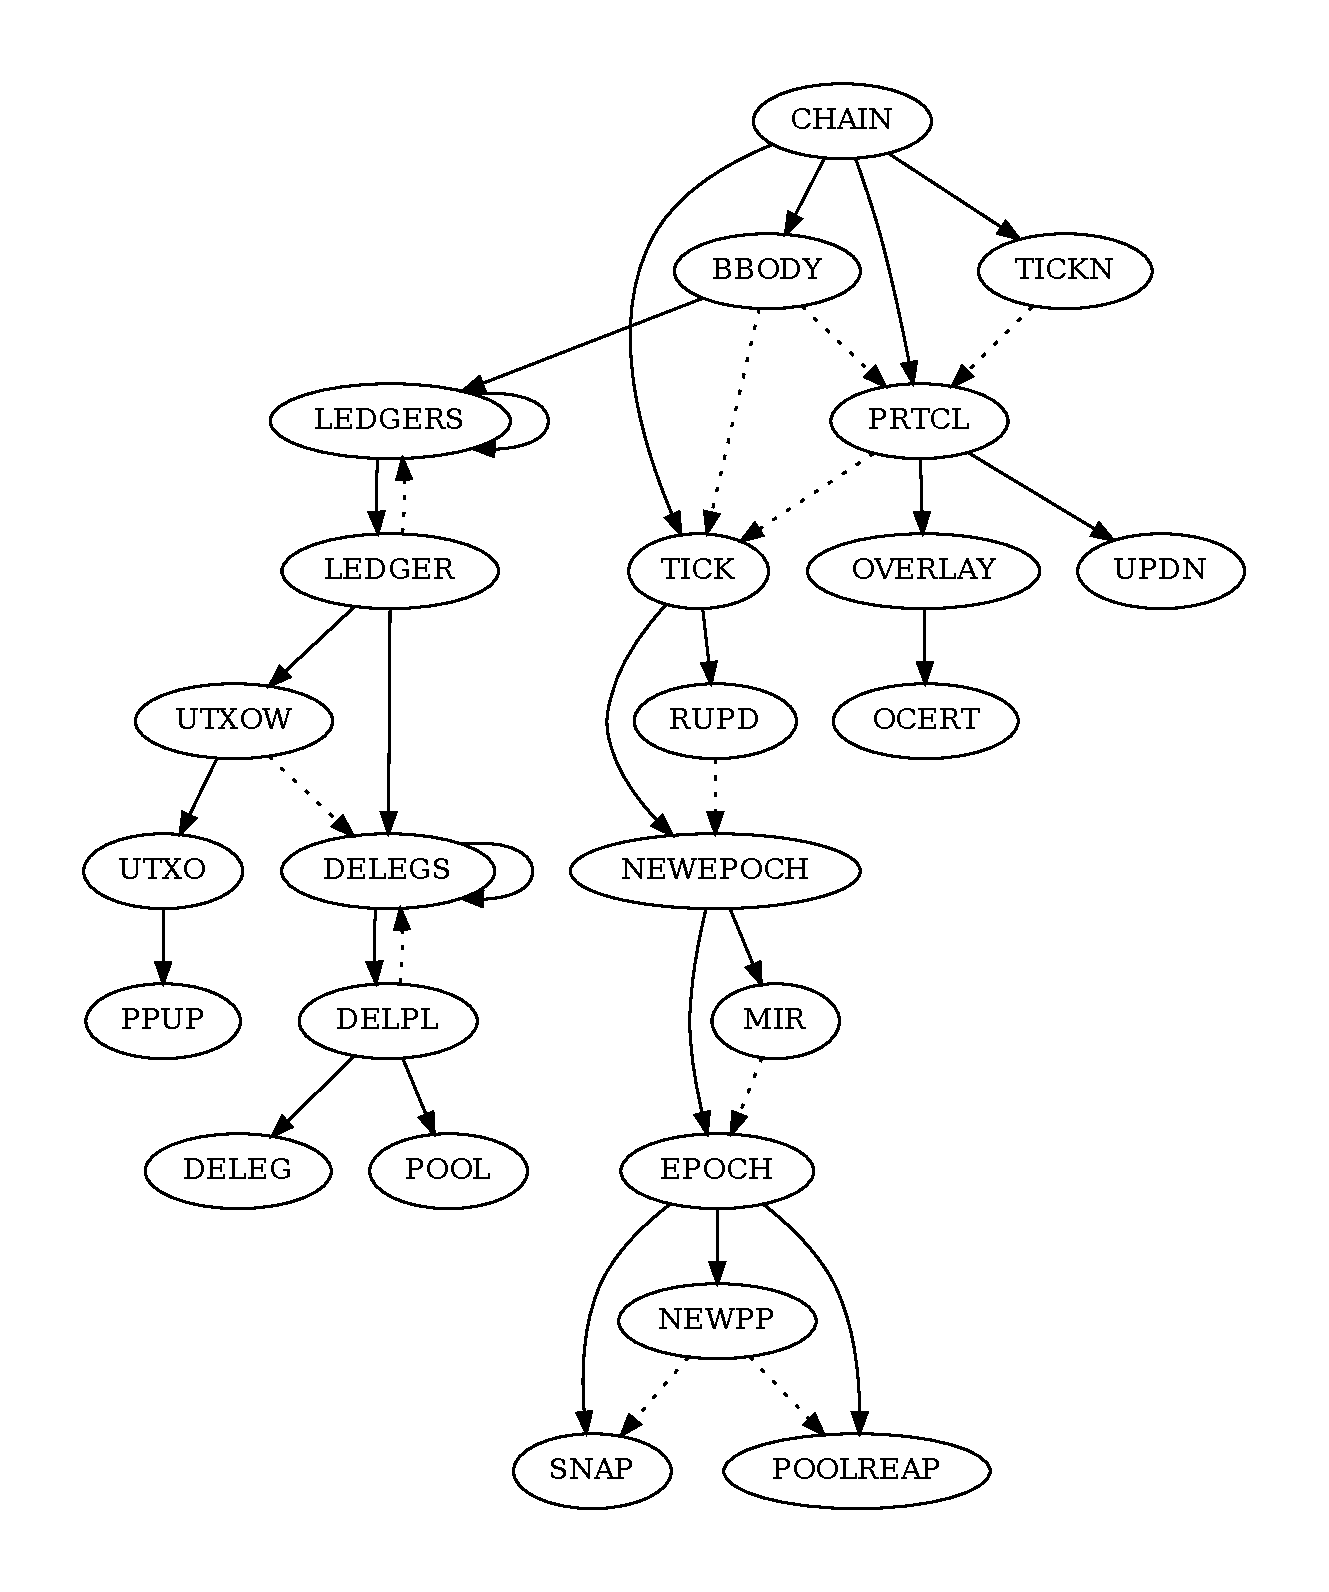
\includegraphics[width=0.6\textwidth]{rules}
\caption{\href{https://hydra.iohk.io/build/18363060/download/1/ledger-spec.pdf\#figure.78}{Figure~78} ``STS Rules, Sub-Rules and Dependencies'' from the Cardano Ledger Spec.}
\label{fig:ledger:spec:78}
\end{figure}

We model blockchain abstractions by extending \ScalaI{Core} with \ScalaI{Chain}:

\begin{ScalaBlockSimple}
trait Chain[R[_]] extends Core[R]:
  import TypeInference.given
  
  // ...
end Chain
\end{ScalaBlockSimple}

\noindent The repetition of the \ScalaI{import} statement is necessary due to 
Scala's scoping rules, that is the implicits represented by 
\ScalaI{TypeInference.given} are not automatically inherited from 
\ScalaI{Core} to \ScalaI{Chain}. From now on in this section, we will assume 
that code is within the \ScalaI{Chain} definition, unless explicitly stated 
otherwise. Also, any Figure references in the code correspond to the Cardano 
Ledger Spec (designated in the code as \TextI{ledger-spec}), not this 
document. By necessity, some familiarity with respective notions from the 
Cardano Ledger Spec is necessary, in order to follow this section comfortably.

%%%%%%%%%%%%%%%%%%%%%%%%%%%%%%%%%%%%%%%%%%%%%%%%%%%%%%%%%%%%%%%%%%%%
\subsection{Warm-up}
\label{sec:chain:warmup}
%%%%%%%%%%%%%%%%%%%%%%%%%%%%%%%%%%%%%%%%%%%%%%%%%%%%%%%%%%%%%%%%%%%%

\subsubsection*{\fbox{\ScalaI{GenesisDelegation}}}

We can start with something simple, in fact one of our initial attempts:

\begin{ScalaBlockSimple}
  // fig.2, p.5, ledger-spec
  // Hash of a key
  type KeyHash = String
  type KeyHash_VRF  = KeyHash
  type KeyHash_Pool = KeyHash
  type KeyHash_G    = KeyHash
  
  // fig.12, p.19 ledger-spec
  // genesis delegations
  type GenesisDelegation =
    Map[R[KeyHash_G], R[Pair[R[KeyHash], R[KeyHash_VRF]]]]
\end{ScalaBlockSimple}

\noindent where \ScalaI{String} and \ScalaI{Map} are \ScalaI{Core}'s 
primitive types. You can see successive ``applications'' of \ScalaI{R[_]} to 
compose types from other types, in a bottom-up fashion:
\begin{align*}
\ScalaI{KeyHash}, \enspace \ScalaI{KeyHash_VRF} 
  & \to \ScalaI{R[KeyHash]}, \enspace \ScalaI{R[KeyHash_VRF]} \\
  & \to \ScalaI{Pair[R[KeyHash], R[KeyHash_VRF]]} \\ 
  & \to \ScalaI{R[Pair[R[KeyHash], R[KeyHash_VRF]]]} \\ 
  & \to \ScalaI{Map[R[KeyHash_G], R[Pair[R[KeyHash], R[KeyHash_VRF]]]]} \\
  & \to \ScalaI{GenesisDelegation} \\
  & \to \ScalaI{R[GenesisDelegation]}
\end{align*}

\noindent The ideas of ``bottom-up'' and ``compositional'' are fundamental 
within the context of denotational semantics and tagless-final. We have shown 
it here for types, but it will also be evident in computations.

Please note that we have defined:

\ScalaI{type GenesisDelegation = Map...}

\noindent and not:

\ScalaI{type GenesisDelegation = R[Map...]}. It is easy to see that a 
\ScalaI{Chain} function that needs an instance of \ScalaI{GenesisDelegation} 
will be encoded as:

\ScalaI{def gd_fun(gd: R[GenesisDelegation]): ....}

\noindent and not as:

\ScalaI{def gd_fun(gd: GenesisDelegation): ....}

\noindent \textit{unless} it is the operation that lifts a 
\ScalaI{GenesisDelegation}, so a \ScalaI{Map}, to an \ScalaI{R[_]} value:

\ScalaI{def gd_new(gd: GenesisDelegation): R[GenesisDelegation]}

\noindent in the same way that

\ScalaI{def zat(scala.Int): R[Zat]}

\noindent does the lifting for integers (\ScalaI{Zat} is to $\mathbb{Z}$ what 
\ScalaI{Nat} is to $\mathbb{N}$).

Why \ScalaI{type KeyHash = String} and not some more specific type? In 
particular, this type alias in Scala gives \ScalaI{KeyHash} all the 
\ScalaI{String} operations, so clearly the domain of \ScalaI{String}s is 
leaking into the domain of \ScalaI{KeyHash}es. If \ScalaI{KeyHash = String}, 
can we then use \ScalaI{str_concat()} from \autoref{fig:prim:ops:str} on 
\ScalaI{KeyHash}es? From the point of view of the Scala compiler, we can but 
the domain semantics are wrong. In essence, we need an \ScalaI{opaque} type, 
like what we did in \vref{fig:prim:types:nat} for \ScalaI{Nat}. Nevertheless, 
we presented the approach as being a fast translation from the Cardano Ledger 
Spec figures to some executable Scala, and it has served its purpose well 
towards our proof-of-concept. We have, though, another ace up our sleeve: 
user-defined structs.

%%%%%%%%%%%%%%%%%%%%%%%%%%%%%%%%%%%%%%%%%%%%%%%%%%%%%%%%%%%%%%%%%%%%
\subsection{A little bit further}
\label{sec:chain:further}
%%%%%%%%%%%%%%%%%%%%%%%%%%%%%%%%%%%%%%%%%%%%%%%%%%%%%%%%%%%%%%%%%%%%

\subsubsection*{\fbox{\ScalaI{KESPeriod}}}
The encoding of user-defined structs in its present form is the outcome of a 
deliberate exercise in design. Let's see how we can put them to use for 
ledger semantics. Here is \ScalaI{KESPeriod}:

\begin{ScalaBlockSimple}
  // Bare fields  
  object bf:
    def F[N <: FieldName: ValueOf, F: Ty]: BareField[N, F] = 
      bare_field[N, F]
    
    // A Nat value named "v" in generated code
    val v_Nat = F["v", Nat]
    // ... more bare fields
  end bf
  
  // fig.7, p.13 ledger-spec
  object KESPeriod {
    case class KESPeriodStruct(v: R[Nat]) extends AnyStruct
    val Fields = Tuple1(bf.v_Nat)
    val Constr = struct_constructor[KESPeriodStruct]

    val Struct = def_struct(Fields, Constr)
    val v      = def_field(Struct, bf.v_Nat, _.v)
  }
  type KESPeriod = KESPeriod.KESPeriodStruct

\end{ScalaBlockSimple}

\noindent Here is \ScalaI{Slot}, which we will need shortly, together with 
\ScalaI{KESPeriod}:

\begin{ScalaBlockSimple}
  // Absolute slot
  // p.10 ledger-spec
  object Slot {
    case class SlotStruct(v: R[Nat]) extends AnyStruct
    val Fields = Tuple1(bf.v_Nat)
    val Constr = struct_constructor[SlotStruct]

    val Struct = def_struct(Fields, Constr)
    val v      = def_field(Struct, bf.v_Nat, _.v)
  }
  type Slot = Slot.SlotStruct
\end{ScalaBlockSimple}

\noindent From page 11 of the Cardano Ledger Spec we have the following, 
\textit{emphasis is ours}:
\begin{quote}
Note that \textit{Slot is an abstract type}, while the constants are 
integers. \textit{We use multiplication and division symbols on these 
distinct types without being explicit about the types and conversion}.
\end{quote}
Clearly, there is a difference from the above statement and the approach we 
take here. We are explicit about the types and their operations. ``Explicit'' 
does not mean unable to handle abstractions. The very existence of the direct 
and AST interpretations, as potentially two ends of a spectrum, shows we do 
not shy away from abstractions: they are at the heart of tagless-final.

With \ScalaI{KESPeriod} and \ScalaI{Slot} defined, we can proceed to the 
denotation semantics of the \textsf{KES} period calculation of a slot:

\begin{ScalaBlockSimple}
  // fig.9, p.14 ledger-spec
  // Denotational semantics of: KES period of a slot
  protected def impl_kes_period(slot: R[Slot]): R[KESPeriod] =
    val n_slot = v["n_slot"] := n_of_slot(slot)
    val n_kesp = v["n_kesp"] := n_slot / Slots_Per_KES_Period
    val kesp   = v["kesp"]   := kes_period_of_n(n_kesp)

    kesp
  end impl_kes_period

  lazy val kes_period = f["kes_period"] := p["slot"] --> impl_kes_period
\end{ScalaBlockSimple}
\noindent where:
\begin{ScalaBlockSimple}
  // Absolute slot
  // p.10 ledger-spec
  inline def n_of_slot(s: R[Slot]): R[Nat] = s.get(Slot.v)
  
  // fig.8, p.14 (constants)
  protected def impl_Slots_Per_KES_Period: R[Nat]
  
  lazy val Slots_Per_KES_Period =
    v["Slots_Per_KES_Period"] := impl_Slots_Per_KES_Period
    
  protected def impl_kes_period_of_n(n: R[Nat]): R[KESPeriod] =
    KESPeriod.Struct(Tuple1(n))
  
  lazy val kes_period_of_n =
    f["kes_period_of_n"] := p["n"] --> impl_kes_period_of_n
\end{ScalaBlockSimple}

\noindent Now, \ScalaI{kes_period} is a symbol that can be used anywhere else 
in eDSL-based code that requires the particular calculation. This means that 
\ScalaI{impl_kes_period()} is an implementation detail the eDSL-based user 
code should not care about.

As a side note, the expression \ScalaI{s.get(Slot.v)} typechecks because 
\ScalaI{Slot.v} is a \ScalaI{Slot}'s field that is derived from the bare 
field \ScalaI{bf.v_Nat}. Although the bare field stands on its own and is 
re-usable, \ScalaI{Slot.v} is created in a way that the type of the 
respective struct is attached to it's type, so that it cannot be used in an 
irrelevant context. Using \vref{fig:structs:ops:dot}, \ScalaI{s.get(Slot.v)} 
is desugared to \ScalaI{dot(s, Slot.v)}.

\subsubsection*{\fbox{\ScalaI{pv_can_follow()}}}

As yet another example, we specify the \ScalaI{pv_can_follow()} function:

\begin{ScalaBlockSimple}
  // fig.7, p.13 ledger-spec
  // protocol version
  type ProtVer = Pair[R[Nat] /* m */, R[Nat] /* n */]
  
  // fig.12, p. 19
  protected def impl_pv_can_follow(a: R[ProtVer], b: R[ProtVer]): R[Bool] =
    // (m, n)
    val m  = v["m"] := pair_first(a)
    val n  = v["n"] := pair_second(a)

    // (m_, n_), which is (m', n') in the PDF
    val m_ = v["m_"] := pair_first(b)
    val n_ = v["n_"] := pair_second(b)

    // (m + 1,  0) == (m', n')
    ((m + 1) === m_) && (0 === n_) ||
    // (m,  n + 1) == (m', n')
    (m === m_) && ((n + 1) === n_)
  end impl_pv_can_follow

  lazy val pv_can_follow =
    f["pv_can_follow"] := (p["a"], p["b"]) --> impl_pv_can_follow
\end{ScalaBlockSimple}

\noindent where the \ScalaI{Core} primitive type \ScalaI{Pair} and its 
operations \ScalaI{pair_first()} and \ScalaI{pair_second()} are the 
``expected'' ones:

\begin{ScalaBlockSimple}
  // outside Core
  type Pair[A, B] = (A, B)
  
  trait Core[R[_]]:
    // ...
    def pair_new   [A: Ty, B: Ty](a: R[A], b: R[B]): R[Pair[R[A], R[B]]]
    def pair_first [A: Ty, B: Ty](pair: R[Pair[R[A], R[B]]]): R[A]
    def pair_second[A: Ty, B: Ty](pair: R[Pair[R[A], R[B]]]): R[B]
    // ...
  end Core
\end{ScalaBlockSimple}


%%%%%%%%%%%%%%%%%%%%%%%%%%%%%%%%%%%%%%%%%%%%%%%%%%%%%%%%%%%%%%%%%%%%
%%%%%%%%%%%%%%%%%%%%%%%%%%%%%%%%%%%%%%%%%%%%%%%%%%%%%%%%%%%%%%%%%%%%
\section{The AST-based interpretation}
\label{sec:ast}
%%%%%%%%%%%%%%%%%%%%%%%%%%%%%%%%%%%%%%%%%%%%%%%%%%%%%%%%%%%%%%%%%%%%
%%%%%%%%%%%%%%%%%%%%%%%%%%%%%%%%%%%%%%%%%%%%%%%%%%%%%%%%%%%%%%%%%%%%
If \ScalaI{Core} and \ScalaI{Chain} qualify as the ``front-end'', we 
certainly need to have a look at the ``back-end''. The direct interpretation 
is rather ...direct and we will not present it further in this paper. Here we 
are concerned about our two ASTs. The next section will comment on the code 
generation part.

%%%%%%%%%%%%%%%%%%%%%%%%%%%%%%%%%%%%%%%%%%%%%%%%%%%%%%%%%%%%%%%%%%%%
  \subsection{The first AST}
%%%%%%%%%%%%%%%%%%%%%%%%%%%%%%%%%%%%%%%%%%%%%%%%%%%%%%%%%%%%%%%%%%%%

The first AST  is close to the eDSL and follows the flow of the types via the 
operations. It is a Generalized Algebraic Data Type (GADT):

\begin{ScalaBlockSimple}
enum AST[T](val ty: Ty[T]):
  case ...
  case ...
  // ...
end enum
\end{ScalaBlockSimple}

\noindent It has been introduced to serve the AST-based interpretation:

\begin{ScalaBlockSimple}
trait ASTCore extends Core[AST]:
  // ...
end ASTCore
\end{ScalaBlockSimple}

\noindent where the representation \ScalaI{R[T]} is now fixed to 
\ScalaI{AST[T]}. As a reminder, in the direct representation we have 
\ScalaI{R[T] = Id[T] = T}, so each type is itself. Each node in the AST has a 
type \ScalaI{T} and for that type we require a witness \ScalaI{val ty: 
Ty[T]}. The latter is obtained via the type inference mechanism explained in 
\vref{sec:types}. All primitive operations are modeled as \ScalaI{AST[T]} 
node constructors, where \ScalaI{T} represents the return type of an 
operation.

So, for instance, the \ScalaI{Map} constructor in \ScalaI{Core}:

\begin{ScalaBlockSimple}
  def map_new[K: Ty, V: Ty](): R[Map[R[K], R[V]]]
\end{ScalaBlockSimple}

\noindent is given a direct interpretation of:

\begin{ScalaBlockSimple}
  def map_new[K: Ty, V: Ty](): Map[K, V] = Map()
\end{ScalaBlockSimple}

\noindent For its AST interpretation we just construct the corresponding node:

\begin{ScalaBlockSimple}
  def map_new[K: Ty, V: Ty](): AST[Map[AST[K], AST[V]]] =
    val k_ty = summon[Ty[K]]
    val v_ty = summon[Ty[V]]
    val ty = summon[Ty[Map[AST[K], AST[V]]]]
    
    AST.MapNewT(k_ty, v_ty, ty)
  end map_new
\end{ScalaBlockSimple}

\noindent The \ScalaI{summon[Ty[K]]} Scala~3 built-in \textit{summons a 
witness} for our eDSL's \ScalaI{Ty[K]} inferred type. \ScalaI{MapNewT}, as a 
constructor of the \ScalaI{AST[T]} GADT, is defined as:

\begin{ScalaBlockSimple}
  case MapNewT[K, V](
    k_ty: Ty[K],
    v_ty: Ty[V],
    override val ty: Ty[Map[AST[K], AST[V]]]
  ) extends AST(ty)
\end{ScalaBlockSimple}

For other operations, we proceed in a similar fashion. For instance, binding 
values to names and defining parameters to functions:

\begin{ScalaBlockSimple}
enum AST[T](val ty: Ty[T]):
  // ...
  case BindT[T](
    name: String, value: AST[T],
    override val ty: Ty[T],
    creation: BindTCreation,
    pre_cond: List[AST[?]] = Nil,
    post_cond: List[AST[?]] = Nil
  ) extends AST(ty)
  
  case ParamT[T](name: String, override val ty: Ty[T]) extends AST(ty)
  // ...
end AST
\end{ScalaBlockSimple}

\noindent or representing properties, functions, and function application:

\begin{ScalaBlockSimple}
enum AST[T](val ty: Ty[T]):
  // ...
  
  case PropT(prop: Prop[AST]) extends AST(Ty.PropTy[AST]())
  
  case Fun1T[A, Z](
    a: ParamT[A],
    f_applied: () => AST[Z], // f(a), computed on demand
    f: Fun1[AST, A, Z],
    override val ty: Ty[Fun1[AST, A, Z]]
  ) extends AST(ty)

  case App1T[A, Z](
    f: AST[Fun1[AST, A, Z]],
    a: AST[A],
    override val ty: Ty[Z]
  ) extends AST(ty)
  // ...
end AST
\end{ScalaBlockSimple}

\noindent Even our fold (see \autoref{sec:prim:ops}) gets its node:

\begin{ScalaBlockSimple}
  case SeqFoldLeftT[K, L](
    seq: AST[Seq[AST[K]]],
    initial: AST[L],
    f: AST[Fun2[AST, L, K, L]],
    k_ty: Ty[K],
    l_ty: Ty[L]
  ) extends AST(l_ty)
\end{ScalaBlockSimple}

\noindent Interpreting \ScalaI{seq_fold_left()} of \vref{fig:prim:ops:seq} in 
the \ScalaI{AST[T]}-based semantics requires building the proper node:

\begin{ScalaBlockSimple}
  def seq_fold_left[K: Ty, L: Ty](
    seq: AST[Seq[AST[K]]],
    initial: AST[L],
    f: AST[Fun2[AST, L, K, L]]
  ): AST[L] =
  
    val k_ty = summon[Ty[K]]
    val l_ty = summon[Ty[L]]

    SeqFoldLeftT(seq, initial, f, k_ty, l_ty)
  end seq_fold_left
\end{ScalaBlockSimple}

\subsubsection*{Introspection, recursion and laziness}
A usual ``complaint'' about tagless-final is we cannot introspect into the 
function bodies. For the \ScalaI{Core} operation:

\begin{ScalaBlockSimple}
def fun1[A: Ty, Z: Ty](a: Name, f: Fun1[R, A, Z]): R[Fun1[R, A, Z]]
\end{ScalaBlockSimple}

\noindent the direct interpretation can be as straightforward as:

\begin{ScalaBlockSimple}
def fun1[A: Ty, Z: Ty](a: Name, f: Fun1[Id, A, Z]): Fun1[Id, A, Z] = f
\end{ScalaBlockSimple}

\noindent or, in its desugared form:

\begin{ScalaBlockSimple}
def fun1[A: Ty, Z: Ty](a: Name, f: A => Z): A => Z = f
\end{ScalaBlockSimple}

\noindent It is clear that in the usual direct interpretation an eDSL 
function is just a lambda abstraction from the meta language, so one does not 
have access to the function body.

But introspection \textit{is} possible, and the trick is to craft a 
representation that helps towards this direction, in our case 
\ScalaI{AST[T]}. An \ScalaI{AST[T]} node is a value that we can look at and 
manipulate at runtime. We'll also add some more ingredients along the way:

\begin{ScalaBlockLines}
  def fun1[A: Ty, Z: Ty](a_name: Name, f: Fun1[AST, A, Z]):
    AST[Fun1[AST, A, Z]] =
    
    val a_ty = summon[Ty[A]]
    val ty   = summon[Ty[Fun1[AST, A, Z]]]

    val a: ParamT[A] = ParamT[A](a_name, a_ty)
    val f_applied = () => f(a)

    Fun1T(a, f_applied, f, ty)
  end fun1
\end{ScalaBlockLines}

\noindent The crucial details are in the two lines 7 and 8 above. We 
synthesize a parameter \ScalaI{a} of the correct type and then we apply the 
function \ScalaI{f} to the parameter, albeit in a \textit{delayed} fashion, 
as \ScalaI{() => f(a)} indicates. Now, \ScalaI{f_applied} can compute the 
body of the function! The reason we do not do that in an immediate way:

\begin{ScalaBlockSimple}
val f_applied = f(a)
\end{ScalaBlockSimple}

\noindent is to avoid an infinite loop if the respective function calls 
itself. By taking into account the discussion of \vref{sec:rec:fun}, 
everything is in place for introspecting all details of an \ScalaI{AST[T]} 
node, including recursive function definitions. Furthermore, pattern-matching 
does not need any machinery other than the \ScalaI{AST[T]} nodes themselves. 
This leads us to the second AST.

%%%%%%%%%%%%%%%%%%%%%%%%%%%%%%%%%%%%%%%%%%%%%%%%%%%%%%%%%%%%%%%%%%%%
\subsection{The second AST}
%%%%%%%%%%%%%%%%%%%%%%%%%%%%%%%%%%%%%%%%%%%%%%%%%%%%%%%%%%%%%%%%%%%%
There are various reasons for the introduction of a second AST:

\begin{itemize}
  \item The fully typed \ScalaI{AST[T]} is deliberately close to the syntax 
  that \ScalaI{Core} exposes via its operations: conceptually, it is almost a 
  \textit{concrete} instead of an \textit{abstract} syntax tree. A code 
  generator does not necessarily need the information in the same form. For 
  instance, information can be consolidated:

  \begin{itemize}
      \item Combinations of \ScalaI{BindT} (\autoref{fig:prim:ops:bind}) with 
      \ScalaI{Fun1T}, \ScalaI{Fun2T} etc. (\autoref{fig:prim:types:fun} and 
      \autoref{fig:prim:ops:fun}) can be collapsed to one \ScalaI{FunDefT} 
      node for function definitions. Generating code from one such general 
      function definition ensures that the right code is concentrated in one 
      place. We will show \ScalaI{FunDefT} shortly.
      
      \item Binary operations that are represented by different 
      \ScalaI{AST[T]} nodes, such as \ScalaI{BoolBinOpT} for boolean logic 
      operators (\textsf{or}, \textsf{and}), \ScalaI{ComparisonBinOpT} for 
      comparison operators ($<$, $=$), and \ScalaI{ArithBinOpT} for 
      arithmetic operators ($+$, $*$), can all be represented by one 
      \ScalaI{BinOpExprT} node. We will show \ScalaI{BinOpExprT} shortly.
  \end{itemize}
  
  \item While the ``frontend'' (eDSL) does not separate bindings for 
  functions from bindings for non-functions, a code generation backend may 
  need to know which case it is dealing with because code can look different 
  in each case. For instance, in Scala, we may emit a \ScalaI{def} for a 
  function (method) and a \ScalaI{val} for other variables. The eDSL, though, 
  models \ScalaI{bind()}-ings without distinction, and this is a feature. So 
  some post-processing of the \ScalaI{AST[T]} may be needed.

  \item At some point we realized that our code generation framework for 
  Scala became too tangled to the rest of the \ScalaI{AST[T]}-related code 
  (post-)processing. What if we needed to introduce a code generator for 
  another language? This is of course ``Software Engineering 101'' but in any 
  case, the power of a Minimum Viable Product (MVP) cannot be 
  under-estimated. Our code generation library was using a visitor already. 
  This is a modular approach but only as far as the \textit{unprocessed 
  input} is concerned: given \ScalaI{AST[T]} nodes as input, if you need to 
  transform it before producing the code generation output, then a good 
  strategy is to write the transformation and code generation as two separate 
  operations that are composed together in a modular way.
  
  \item When generating code for a target language, there are constructs that 
  the backend needs to generate, which do not exist in the frontend in a 
  literal form. For instance, \ScalaI{import} statements or all the primitive 
  type and operations definitions. There is no corresponding \ScalaI{AST[T]} 
  node for them, so we need a new construct.
\end{itemize}
 
\noindent The above led to our second AST, \ScalaI{CGTree}, where the 
\ScalaI{CG} prefix stands for \textit{Code Generation}. \ScalaI{CGTree} is a 
\textit{simple} ADT, not a GADT:

\begin{ScalaBlockSimple}
enum CGTree:
  // Expressions (user-defined)
  case LiteralExprT(value: Literal)
  case BinOpExprT  (op: BinOp,   a: CGTree, b: CGTree)
  case CallExprT   (f: CGTree, types: Tys, args: CGTrees)
  // ...

  // Struct operations
  case StructNewExprT(name: String, fields: NameCGTrees)
  case DotExprT      (prefix: CGTree, field: NameType)
  
  // Definitions
  // val name: ty = value 
  case ValDefT(name_ty: NameType, value: CGTree, is_lazy: Bool)
  // def name(params): ret_ty = body
  case FunDefT(
    name: String,
    params: NameTypes,
    ret_ty: Ty[?],
    body: CGTrees,
    inline_is: InlineIs,
    pre_cond: List[CGProp],
    post_cond: List[CGProp]
  )

  // ...
end CGTree
\end{ScalaBlockSimple}

\noindent where we can see the previously mentioned \ScalaI{FunDefT} and 
\ScalaI{BinOpExprT}. The full definition can be found in the source code 
repository.

%%%%%%%%%%%%%%%%%%%%%%%%%%%%%%%%%%%%%%%%%%%%%%%%%%%%%%%%%%%%%%%%%%%%
%%%%%%%%%%%%%%%%%%%%%%%%%%%%%%%%%%%%%%%%%%%%%%%%%%%%%%%%%%%%%%%%%%%%
\section{Code generation}
\label{sec:code:gen}
%%%%%%%%%%%%%%%%%%%%%%%%%%%%%%%%%%%%%%%%%%%%%%%%%%%%%%%%%%%%%%%%%%%%

\newcommand{\codeIN}{\ensuremath{\textsfi{code}_\textsfi{IN}}\xspace}
\newcommand{\codeOUT}{\ensuremath{\textsfi{code}_\textsfi{OUT}}\xspace}
\newcommand{\visitorAST}{\ensuremath{\textsfi{Visitor}_\textsfi{AST[T]}}\xspace}
\newcommand{\visitorCGTree}{\ensuremath{\textsfi{Visitor}_\textsfi{CGTree}}\xspace}

\begin{figure}[tb]
\centering
\fbox{\codeIN} $\xrightarrow{\textsfi{eDSL}}$ %
\fbox{\ScalaI{AST[T]}} $\xrightarrow{\visitorAST}$ %
\fbox{\ScalaI{CGTree}} $\xrightarrow{\visitorCGTree}$ %
\fbox{\codeOUT}
\caption{Code generation end-to-end pipeline.}
\label{fig:ast:pipeline}
\hrulefill
\end{figure}

We mentioned that we use the visitor pattern to process \ScalaI{AST[T]} 
nodes. We do the same for \ScalaI{CGTree} nodes. The respective end-to-end 
pipeline is shown in \vref{fig:ast:pipeline}. Both \codeIN and \codeOUT are 
Scala~3 in our case. The choice for \codeIN is rigid and has already been 
made in the context of the present work, since our eDSL design is using 
Scala~3 for the role of the meta language. On the other hand, in the current 
design the choice for \codeOUT is completely open. We just picked Scala~3 
again, in order to be able to directly compare eDSL code with generated code 
\textit{for the same semantics definition}. \autoref{fig:ast:pipeline} is 
also related to \vref{fig:commutative-diagram}. 

%%%%%%%%%%%%%%%%%%%%%%%%%%%%%%%%%%%%%%%%%%%%%%%%%%%%%%%%%%%%%%%%%%%%
\subsection{Dependencies}
%%%%%%%%%%%%%%%%%%%%%%%%%%%%%%%%%%%%%%%%%%%%%%%%%%%%%%%%%%%%%%%%%%%%

In going from \ScalaI{AST[T]} to \ScalaI{CGTree}, we use \visitorAST 
implementations more than once. The obvious goal is of course to create 
\ScalaI{CGTree} nodes. In order to do this cleanly in one pass, we re-use the 
visitor infrastructure once more (but with a different implementation) to 
compute some needed dependencies. Let's see how this relates to binding names 
to values and the subtle dependency details we need to handle. Remember 
(\vref{sec:bind}) that we have chosen for eDSL code to resemble 
\textit{standard} Scala code as much as possible, so binding is done with 
\ScalaI{:=}, an extension method delegating to \ScalaI{Core}'s 
\ScalaI{bind()} (\vref{fig:prim:ops:bind}).

\begin{ScalaBlockSimple}
  def impl_duration_of_slots(a: R[Slot], b: R[Slot]): R[Duration] =
    val n_a  = v["n_a"]  := n_of_slot(a)
    val n_b  = v["n_b"]  := n_of_slot(b)
    val diff = v["diff"] := n_b - n_a

    Duration.Struct(Tuple1(diff))
  end impl_duration_of_slots

  lazy val duration_of_slots =
    f["duration_of_slots"] := (p["a"], p["b"]) --> impl_duration_of_slots
\end{ScalaBlockSimple}

\noindent where \ScalaI{Duration} is defined like \ScalaI{Slot} 
(\vref{sec:chain:further}):

\begin{ScalaBlockSimple}
  // fig.7, p.13 ledger-spec
  object Duration {
    case class DurationStruct(v: R[Nat]) extends AnyStruct
    // ...
  }
  type Duration = Duration.DurationStruct
\end{ScalaBlockSimple}

\noindent and \ScalaI{n_of_slot()} translates a \ScalaI{Slot} to a 
\ScalaI{Nat} (again, \autoref{sec:chain:further}). In the AST interpretation, 
the body of \ScalaI{duration_of_slots()} essentially%
\footnote{This is not an exact string representation of the AST, we omit or 
change some details in order to save space, without compromising on the 
essence.}%
 is this \ScalaI{AST[T]} node:

\begin{ScalaBlockLines}
StructNewT[Duration](
  BindT[Nat](
    "diff",
    ArithBinOpT[Nat](
      "-",
      BindT[Nat](
        "n_b",
        StructDotT[Slot, Slot.v](
          ParamT[Slot]("b"),
          Slot.v
        )
      )
      BindT[Nat](
        "n_a",
        StructDotT[Slot, Slot.v](
          ParamT[Slot]("a"),
          Slot.v
        )
      )
    )
  )
)
\end{ScalaBlockLines}

So, in the eyes of the visitor, the body of \ScalaI{duration_of_slots()} is 
just one expression! Where have the \ScalaI{val} statements gone? Simply, 
there are no statements, we only have type-full expressions linked to other 
expressions. Clearly, we need to process these expressions further, in order 
to recover the original intention of the programmer. We need to calculate 
dependencies \textit{and} make sure we emit them in the correct order: This 
is exactly what the second \visitorAST does. The net result of the 
compositions of the two visitors is a list of \ScalaI{CGTree} nodes, which 
represent the (re)generated body of \ScalaI{duration_of_slots()}:

\begin{ScalaBlockLines}
List(
  ValDefT(                         val n_a = v["n_a"] := n_of_slot(a)
    "n_a", NatTy,
    DotExprT(
      RefT("a", StructTy[Slot]),
      Slot.v, NatTy
    )
  ),

  ValDefT(                         val n_b = v["n_b"] := n_of_slot(b)
    "n_b", NatTy,
    DotExprT(
      RefT("b", StructTy[Slot]),
      Slot.v, NatTy
    )
  ),

  ValDefT(                         val diff = v["diff"] := n_b - n_a
    "diff", NatTy,
    BinOpExprT(
      "-",
      RefT("n_b", NatTy),
      RefT("n_a", NatTy)
    )
  ),
  
  StructNewExprT(                  Duration.Struct(Tuple1(diff))
    "Duration",
    RefT("diff", NatTy)
  )
)
\end{ScalaBlockLines}

\noindent Now we have clear definitions for \ScalaI{n_a}, \ScalaI{n_b} and 
\ScalaI{diff}, and any reference to them is given by a \ScalaI{RefT()} node. 
The resemblance to the specification of \ScalaI{duration_of_slots()}, with 
respective fragments copied on the right column, is clear. Note also how we 
have gone from a fully typed AST node (\ScalaI{BindT[Nat]()}), to a node 
where the type is represented only by its witness at the value level 
(\ScalaI{ValDefT(NatTy)}). The former is an \ScalaI{AST[T]} node, the latter 
is a \ScalaI{CGTree} node.

%%%%%%%%%%%%%%%%%%%%%%%%%%%%%%%%%%%%%%%%%%%%%%%%%%%%%%%%%%%%%%%%%%%%
\subsection{Primitive operations}
%%%%%%%%%%%%%%%%%%%%%%%%%%%%%%%%%%%%%%%%%%%%%%%%%%%%%%%%%%%%%%%%%%%%
We know that the \ScalaI{Core} requires, among other things, the presence of 
an addition operator for the \ScalaI{Nat} type, but how do we make sure a 
particular code generator will provide it? The best we can do is to simply 
enumerate all the requirements to the generator, so that at least there is no 
excuse about forgetting to emit some code. This is the role of the 
\ScalaI{PrimFun} \ScalaI{enum}:

\begin{ScalaBlockSimple}
enum PrimFun:
  case Nat           // Nat constructor
  case Str_Len       // length of a string
  case Map_New       // Map constructor
  case Map_Put       // Map.put(key, value) operation
  case Seq_Fold_Left // (left) fold is a primitive !
  // ...
end PrimFun
\end{ScalaBlockSimple}

\noindent Then, we require that each code generator implements a 
corresponding visitor for primitive operations:

\begin{ScalaBlockSimple}
abstract class PrimFunVisitor:
  type Ctx = SourceCodeWriter
  type Result = Unit

  def visit_Nat(pf: PrimFun, ctx: Ctx): Result
  def visit_Str_Len(pf: PrimFun, ctx: Ctx): Result
  def visit_Map_New(pf: PrimFun, ctx: Ctx): Result
  def visit_Map_Put(pf: PrimFun, ctx: Ctx): Result
  def visit_Seq_Fold_Left(pf: PrimFun, ctx: Ctx): Result
  
  // ...
end PrimFunVisitor
\end{ScalaBlockSimple}

%%%%%%%%%%%%%%%%%%%%%%%%%%%%%%%%%%%%%%%%%%%%%%%%%%%%%%%%%%%%%%%%%%%%
\subsection{Properties}
%%%%%%%%%%%%%%%%%%%%%%%%%%%%%%%%%%%%%%%%%%%%%%%%%%%%%%%%%%%%%%%%%%%%
Each property is compiled to its own function, where a proper 
\ScalaI{require()} or \ScalaI{ensure()} is emitted, depending on whether this 
is a pre- or a post- condition. Using the \ScalaI{leftpad()} definitions from 
\autoref{sec:properties}, we now come full circle with everything: from the 
original description to the generated code:

%%%%%%%%%%%%%%%%%%%%%%%%%%%%%%%%%%%%%%%%%%%%%%%%%%%%%%%%%%%%%%%%%%%%
\subsubsection*{Precondition 1: \leftpadprea}
\begin{ScalaBlockSimple}
 def leftpad_pre_cond1(s: String, n: Nat, c: Char): Unit = 
  val n_upper_value: Nat = n
  val n_lower_value: Nat = nat(0)
  
  require(
    (n_upper_value >= n_lower_value),
    "require(n_upper_value >= n_lower_value)"
  )
end leftpad_pre_cond1 //(s: String, n: Nat, c: Char): Unit
\end{ScalaBlockSimple}


%%%%%%%%%%%%%%%%%%%%%%%%%%%%%%%%%%%%%%%%%%%%%%%%%%%%%%%%%%%%%%%%%%%%
\subsubsection*{Postcondition 1: \leftpadposta}
\begin{ScalaBlockSimple}
def leftpad_post_cond1(s: String, n: Nat, c: Char, result: String): Unit = 
  val res_length: Nat = str_len(result)
  val s_length: Nat = str_len(s)
  
  ensure(
    (res_length == nat_max(n, s_length)),
    "ensure(res_length == nat_max(n, s_length))"
  )
end leftpad_post_cond1 //(s: String, n: Nat, c: Char, result: String): Unit
\end{ScalaBlockSimple}

%%%%%%%%%%%%%%%%%%%%%%%%%%%%%%%%%%%%%%%%%%%%%%%%%%%%%%%%%%%%%%%%%%%%
\subsubsection*{Postcondition 2: \leftpadpostb}
\begin{ScalaBlockSimple}
def leftpad_post_cond2(s: String, n: Nat, c: Char, result: String): Unit = 
  val lower: Nat = nat(0)
  val pad_length: Nat = nat_max(nat(0), (n - str_len(s)))
  val upper: Nat = pad_length

  for i <- lower until upper do
    val result_i: Char = str_char_at(result, i)

    ensure(
      char_eq(c, result_i),
      "ensure(char_eq(c, result_i))"
    )
  end for
end leftpad_post_cond2 //(s: String, n: Nat, c: Char, result: String): Unit
\end{ScalaBlockSimple}


The fact that with the AST interpretation we can fully manipulate code that 
we write in \ScalaI{Core} or \ScalaI{Chain} cannot be understated. Note, for 
instance, how the \ScalaI{require()} and \ScalaI{ensure()} calls give, as 
their string description, the very requirement expression itself. In this 
particular case we use the code generator twice or, more precisely, the code 
generator (re)uses itself.


%%%%%%%%%%%%%%%%%%%%%%%%%%%%%%%%%%%%%%%%%%%%%%%%%%%%%%%%%%%%%%%%%%%%
%%%%%%%%%%%%%%%%%%%%%%%%%%%%%%%%%%%%%%%%%%%%%%%%%%%%%%%%%%%%%%%%%%%%
\section{Concluding remarks}
\label{sec:conclusions}
%%%%%%%%%%%%%%%%%%%%%%%%%%%%%%%%%%%%%%%%%%%%%%%%%%%%%%%%%%%%%%%%%%%%
%%%%%%%%%%%%%%%%%%%%%%%%%%%%%%%%%%%%%%%%%%%%%%%%%%%%%%%%%%%%%%%%%%%%
We have presented a pragmatic way where day-to-day software engineering can 
go hand~in~hand with semantics engineering. This is just the tip of the 
iceberg. We believe that we need languages and environments, where semantics 
notions truly unite with the usual programming notions and are first-class. 
But this is a few PhDs (or software engineering milestones or both) further 
down the road\dots

\paragraph*{Transition systems} In the code-base\todo{Where?}, there is an 
initial design for supporting state transition systems, as those described in 
the Cardano Ledger Spec. Historically, after having picked 
\fbox{\textsf{UTxO}}, as explained at the beginning of \autoref{sec:chain}, 
we started with a high-level design that can model any box in 
\autoref{fig:ledger:spec:78}, and then reasoned backwards to see what 
\ScalaI{Core} and \ScalaI{Chain} should look like. The transition system 
design should work with the direct interpretation but we have not extracted 
respective primitives in order to support the AST interpretation, and so, 
code generation. This observation leads us to some comments for more future 
work.

\paragraph*{Some future work}
The list is by no means exhaustive, it is just indicative.
\begin{itemize}
  \item The eDSL is comprehensive, yet still incomplete. More constructs 
  could be provided.
  
  \item The Scala code generator needs to be a bit more robust. Also some 
  implementations need to be filled in.
  
  \item We could explore creating more code generators, for instance WASM and 
  JavaScript would be useful, given the ubiquitous nature of the Web and the 
  amount of software that has started targeting these technologies.
  
  \item Another dimension to consider for code generators is about theorem 
  provers, model checkers and all this family of formal systems. We could 
  also support more property types, for instance invariants.
  
  \item All the ingredients for generating property test suites for 
  ScalaCheck are in place, so an implementation should be straightforward. In 
  fact, the code-base already includes an extension of \ScalaI{Core} with 
  proper generators for some \ScalaI{Core} types.
\end{itemize}

%%%%%%%%%%%%%%%%%%%%%%%%%%%%%%%%%%%%%%%%%%%%%%%%%%%%%%%%%%%%%%%%%%%%
%%%%%%%%%%%%%%%%%%%%%%%%%%%%%%%%%%%%%%%%%%%%%%%%%%%%%%%%%%%%%%%%%%%%
\section{Acknowledgments}
%%%%%%%%%%%%%%%%%%%%%%%%%%%%%%%%%%%%%%%%%%%%%%%%%%%%%%%%%%%%%%%%%%%%
%%%%%%%%%%%%%%%%%%%%%%%%%%%%%%%%%%%%%%%%%%%%%%%%%%%%%%%%%%%%%%%%%%%%
I would like to thank Vincent Hanquez, Director of Creative Engineering at 
IOHK, for embracing, sponsoring and prioritizing this project, and for useful 
discussions during its development. I would also like to thank Nicholas 
Clarke, Javier Diaz and Andre Knispel who answered my initial questions 
regarding the Cardano Ledger Spec, the Haskell implementation and the 
Isabelle formalization.

%%%%%%%%%%%%%%%%%%%%%%%%%%%%%%%%%%%%%%%%%%%%%%%%%%%%%%%%%%%%%%%%%%%%
%%%%%%%%%%%%%%%%%%%%%%%%%%%%%%%%%%%%%%%%%%%%%%%%%%%%%%%%%%%%%%%%%%%%
\bibliographystyle{plain}
\bibliography{report}


%%%%%%%%%%%%%%%%%%%%%%%%%%%%%%%%%%%%%%%%%%%%%%%%%%%%%%%%%%%%%%%%%%%%
%%%%%%%%%%%%%%%%%%%%%%%%%%%%%%%%%%%%%%%%%%%%%%%%%%%%%%%%%%%%%%%%%%%%
\clearpage
%\hrulefill
\appendix

%%%%%%%%%%%%%%%%%%%%%%%%%%%%%%%%%%%%%%%%%%%%%%%%%%%%%%%%%%%%%%%%%%%%
%%%%%%%%%%%%%%%%%%%%%%%%%%%%%%%%%%%%%%%%%%%%%%%%%%%%%%%%%%%%%%%%%%%%
\section{Appendix}
\label{sec:appendix}
%%%%%%%%%%%%%%%%%%%%%%%%%%%%%%%%%%%%%%%%%%%%%%%%%%%%%%%%%%%%%%%%%%%%
%%%%%%%%%%%%%%%%%%%%%%%%%%%%%%%%%%%%%%%%%%%%%%%%%%%%%%%%%%%%%%%%%%%%

\subsection*{Types and data supporting user-defined structs}

%\begin{figure}[t]
\begin{ScalaBlockSimple}
type FieldName = Name /*& Singleton*/

// Marker trait for user-defined structs
trait AnyStruct extends Product

case class StructDef[
  Struct <: AnyStruct,
  // definition of fields, as obtained from new_bare_field()
  Fields <: Tuple,
  // constructor, as obtained from struct_constructor()
  Args   <: Tuple
](
  name: Name,
  ty: Ty[Struct],
  fields: Fields,
  constr: Args => Struct
)

type StructDefs = List[StructDef[?, ?, ?]]

case class FieldDef[
  Struct <: AnyStruct,
  N <: FieldName,
  F,
  R[_]
](struct: StructDef[Struct, _ <: Tuple, _ <: Tuple],
  field: BareField[N, F],
  getter: Struct => R[F]
)

case class BareField[N <: FieldName, F](name: N, ty: Ty[F])
\end{ScalaBlockSimple}
%\caption{Types and data supporting user-defined structs.}
%\label{fig:structs:types}
%\hrulefill
%\end{figure}

\subsection*{Operations supporting user-defined structs}

%\begin{figure}[tb]
\begin{ScalaBlockSimple}
trait Core[R[_]]:
  // ...
  import scala.deriving.Mirror
  
  def bare_field[N <: FieldName: ValueOf, F:Ty]: BareField[N,F] =
    BareField(valueOf[N], summon[Ty[F]])
  
  transparent inline def struct_constructor[Struct <: AnyStruct](
    using StructM: Mirror.ProductOf[Struct]
  ) =
    StructM.fromProduct(_: StructM.MirroredElemTypes)
    
  transparent inline def struct_constructor[Struct <: AnyStruct](
    using StructM: Mirror.ProductOf[Struct]
  ) =
    StructM.fromProduct(_: StructM.MirroredElemTypes)
  
  transparent inline def def_struct[Struct <: AnyStruct : Ty,
    Fields <: Tuple, Args <: Tuple
  ](
    fields: Fields,
    constr: Args => Struct
  ): StructDef[Struct, Fields, Args] =
    val struct_ty = summon[Ty[Struct]]
    val name = struct_ty.repr
    
    StructDef(name, struct_ty, fields, constr)
  end def_struct
  
  transparent inline def def_field[Struct <: AnyStruct,
    Fields <: Tuple, Args <: Tuple, N <: FieldName, F
  ](
    struct: StructDef[Struct, Fields, Args],
    field: BareField[N, F],
    getter: Struct => R[F]
  ): FieldDef[Struct, N, F, R] =
    FieldDef(struct, field, getter)
  end def_field
  // ...
end Core
\end{ScalaBlockSimple}
%\caption{Operations supporting user-defined structs.}
%\label{fig:structs:ops}
%\hrulefill
%\end{figure}

\subsection*{Instantiating user-defined structs}

%\begin{figure}[tb]
\begin{ScalaBlockSimple}
trait Core[R[_]]:
  // ...
  def struct_new[
    Struct <: AnyStruct: Ty,
    Fields <: Tuple,
    Args <: Tuple
  ](
    struct_def: StructDef[Struct, Fields, Args],
    args: Args
  ): R[Struct] /* implementation is R[_]-specific */

  // struct(field_def)
  extension [
    Struct <: AnyStruct: Ty,
    Fields <: Tuple,
    Args <: Tuple
  ](struct_def: StructDef[Struct, Fields, Args])
    def apply(args: Args): R[Struct] =
      struct_new(struct_def, args)
  // ...
end Core
\end{ScalaBlockSimple}
%\caption{Instantiating user-defined structs.}
%\label{fig:structs:ops:new}
%\hrulefill
%\end{figure}

\subsection*{Accessing fields of user-defined structs}

%\begin{figure}[tb]
\begin{ScalaBlockSimple}
trait Core[R[_]]:
  // ...
  // struct.dot(field_def)
  def dot[Struct <: AnyStruct: Ty, N <: FieldName, F: Ty](
    struct: R[Struct],
    field_def: FieldDef[Struct, N, F, R]
  ): R[F]

  // struct.get(field_def)
  extension [Struct <: AnyStruct: Ty](struct: R[Struct])
    def get  [N <: FieldName, F: Ty](
      field_def: FieldDef[Struct, N, F, R]
    ): R[F] = dot(struct, field_def)
    
  // field_def(struct)
  extension [Struct <: AnyStruct: Ty, N <: FieldName, F: Ty](
    field_def: FieldDef[Struct, N, F, R])
    def apply(struct: R[Struct]): R[F] = struct(field_def)
  // ...
end Core
\end{ScalaBlockSimple}
%\caption{Accessing fields of user-defined structs.}
%\label{fig:structs:ops:dot}
%\hrulefill
%\end{figure}


%%%%%%%%%%%%%%%%%%%%%%%%%%%%%%%%%%%%%%%%%%%%%%%%%%%%%%%%%%%%%%%%%%%%
%%%%%%%%%%%%%%%%%%%%%%%%%%%%%%%%%%%%%%%%%%%%%%%%%%%%%%%%%%%%%%%%%%%%

\subsection*{Primitive operations for properties}

%\begin{figure}[tb]
\begin{ScalaBlockSimple}
trait Core[R[_]]:
  // ...
  def prop(p: Prop[R]): R[Prop[R]]

  // This is meant to be used internally, as a building block block for the eDSL itself, not programs using the eDSL.
  // TODO enforce the nature of its use via Scala facilities.
  // See also AST transformation and code generation for properties.
  def prop_bool(expr: R[Bool]): R[Prop[R]] =
    prop( Prop.BoolP(expr) )
  end prop_bool

  // This is meant to be used internally, as a building block block for the eDSL itself, not programs using the eDSL.
  // TODO enforce the nature of its use via Scala facilities.
  // See also AST transformation and code generation for properties.
  def prop_forall_in[X <: (Nat | Zat) : Ty](
    name: Name,
    bounds: (R[X], R[X]),
    upper_bound_is: BoundIs,
    predicate: Fun1[R, X, Bool]
  ): R[Prop[R]] =
    val predicate_f = fun1(name, predicate)
    val ty = summon[Ty[X]]

    prop( Prop.ForAllInRangeP(name, ty, bounds, upper_bound_is, predicate_f) )
  end prop_forall_in

  def prop_forall_in[N <: Name : ValueOf, X <: (Nat | Zat) : Ty](
    bounds: (R[X], R[X]),
    upper_bound_is: BoundIs,
    predicate: Fun1[R, X, Bool]
  ): R[Prop[R]] =
    val name = valueOf[N]
    prop_forall_in(name, bounds, upper_bound_is, predicate)
  end prop_forall_in
  // ...
end Core
\end{ScalaBlockSimple}
%\caption{Primitive operations for properties.}
%\label{fig:props:prim:fun}
%\hrulefill
%\end{figure}



\begin{landscape}

\subsection*{Algorithmic type inference rules, encoded in the logic of Scala implicits, using the Scala~3 \ScalaI{given} syntax}
%\begin{sidewaysfigure}[h]
%\begin{figure}[tb]
\begin{ScalaBlockSimple}
trait TypeInference[R[_]]:
  given given_Unit  : Ty[Unit] = Ty.UnitTy
  given given_NatTy : Ty[Nat]  = Ty.NatTy
  given given_ZatTy : Ty[Zat]  = Ty.ZatTy
  given given_BoolTy: Ty[Bool] = Ty.BoolTy
  given given_StringTy: Ty[String] = Ty.StringTy
  given given_CharTy: Ty[Char] = Ty.CharTy

  given given_RTy[X](using x_ty: Ty[X]): Ty[R[X]] = Ty.RTy(x_ty)

  given given_PropTy: Ty[Prop[R]] = Ty.PropTy[R]()

  given given_Fun0Ty[Z]         (using z: Ty[Z]): Ty[() => Z] =
    Ty.Fun0Ty(z)
  given given_Fun1Ty[A, Z]      (using a: Ty[A], z: Ty[Z]): Ty[(A) => Z] =
    Ty.Fun1Ty(a, z)
  given given_Fun2Ty[A, B, Z]   (using a: Ty[A], b: Ty[B], z: Ty[Z]): Ty[(A, B) => Z] =
    Ty.Fun2Ty(a, b, z)
  given given_Fun3Ty[A, B, C, Z](using a: Ty[A], b: Ty[B], c: Ty[C], z: Ty[Z]): Ty[(A, B, C) => Z] =
    Ty.Fun3Ty(a, b, c, z)
  given given_Fun4Ty[A, B, C, D, Z]   (using a: Ty[A], b: Ty[B], c: Ty[C], d: Ty[D], z: Ty[Z]):
    Ty[(A, B, C, D) => Z] = Ty.Fun4Ty(a, b, c, d, z)
  given given_Fun5Ty[A, B, C, D, E, Z](using a: Ty[A], b: Ty[B], c: Ty[C], d: Ty[D], e: Ty[E], z: Ty[Z]):
    Ty[(A, B, C, D, E) => Z] = Ty.Fun5Ty(a, b, c, d, e, z)

  given given_OptionTy[A]   (using a: Ty[A]          ): Ty[Option[A]]    = Ty.OptionTy(a)
  given given_PairTy  [A, B](using a: Ty[A], b: Ty[B]): Ty[Pair[A, B]]   = Ty.PairTy(a, b)

  given given_MapTy[A, B](using a: Ty[A], b: Ty[B]): Ty[Map[A, B]] = Ty.MapTy(a, b)
  given given_SetTy[A](using a: Ty[A]): Ty[Set[A]] = Ty.SetTy(a)
  given given_SeqTy[A](using a: Ty[A]): Ty[Seq[A]] = Ty.SeqTy(a)

  given [S <: AnyStruct](using tag: ClassTag[S]): Ty[S] = Ty.StructTy(tag)
end TypeInference
\end{ScalaBlockSimple}
%\caption{Algorithmic type inference rules, encoded in the logic of Scala implicits, using the Scala~3 \ScalaI{given} syntax.}
%\label{fig:full-typeinf-rules}
%\hrulefill
%\end{figure}
%\end{sidewaysfigure}
\end{landscape}

\end{document}

